\documentclass[xcolor=dvipsnames]{beamer}
\usetheme{default} 
\usepackage[spanish]{babel} % espanol
\usepackage[utf8]{inputenc} % acentos sin codigo
\usepackage[T1]{fontenc}
\usepackage{array}  % Necesario para el uso de m{} en tabular
\usepackage{graphicx}
\usepackage{eurosym}
\usepackage{xcolor}
\usepackage{colortbl}
\usepackage{pdfpages}
\usepackage{adjustbox}% Necesario si usas imágenes en tu documento

% A SISU beamer based on THU beamer.

% other packages
\usepackage{subcaption}


\usepackage{latexsym,amsmath,xcolor,multicol,booktabs,calligra}
\usepackage{graphicx,pstricks,listings,stackengine}


\setbeamertemplate{section in toc}[sections numbered]


\begin{document}
\AtBeginSection{\frame{\sectionpage}}

\title{Diseño de un modelo neuronal para la detección y la clasificación de intrusiones en redes informáticas}
\author{Hugo López Álvarez \\ Tutor: D. Diego García Álvarez
}
\begin{frame}
    \titlepage
    \begin{figure}[H]
        \begin{center}
            
\includegraphics[width=0.25\linewidth]{img/uva.eps}
        \end{center}
    \end{figure}
\end{frame}

\begin{frame}
    \begin{columns}[t]
        \begin{column}{.45\textwidth}
            \tableofcontents[sections={1-5},sectionstyle=show,subsectionstyle=show/shaded/hide,subsubsectionstyle=show/shaded/hide]
        \end{column}
        \begin{column}{.55\textwidth}
            \tableofcontents[sections={6-10},sectionstyle=show,subsectionstyle=show/shaded/hide,subsubsectionstyle=show/shaded/hide]
        \end{column}
    \end{columns}
\end{frame}
\AtBeginSection[]{
  \sectionframetrue
  \begin{frame}
    \frametitle{Índice}
    \begin{columns}[t]
      \begin{column}{.45\textwidth}
        \tableofcontents[currentsection, sections={1-5}, sectionstyle=show/shaded, subsectionstyle=show/shaded/hide, subsubsectionstyle=show/shaded/hide]
      \end{column}
      \hspace{0.05\textwidth}
      \begin{column}{.55\textwidth}
        \tableofcontents[currentsection, sections={6-10}, sectionstyle=show/shaded, subsectionstyle=show/shaded/hide, subsubsectionstyle=show/shaded/hide]
      \end{column}
    \end{columns}
  \end{frame}
  \sectionframefalse
}

\section{Introducción}
Este documento corresponde con la memoria del Trabajo de Fin de Grado (TFG) del Grado en Ingeniería Informática de la Escuela de Ingeniería Informática (EII) de la Universidad de Valladolid (UVa). Este trabajo se centra en el diseño e implementación de un modelo neuronal capaz de detectar intrusiones en una red informática. El modelo está dividido en dos niveles de clasificación, un modelo de clasificación binaria que clasifica las conexiones como benignas o malignas, y un modelo de clasificación multiclase que recibe como entradas las conexiones clasificadas por el modelo binario como malignas. Este último modelo distingue en nueve tipos diferentes de intrusiones las conexiones que recibe, es decir, trata de determinar el tipo de intrusión. El uso de redes neuronales para la detección de intrusiones permite identificar patrones complejos y no lineales en el tráfico de red, mejorando la capacidad de detectar ataques desconocidos o sofisticados. Además, las redes neuronales pueden adaptarse y aprender continuamente a partir de nuevos datos, aumentando su precisión con el tiempo.

%La principal ventaja de utilizar un modelo neuronal para la detección de intrusiones en una red, frente a los algoritmos tradicionales (como firmas basadas en reglas o análisis estadísticos), radica en su capacidad para aprender patrones complejos y no lineales en los datos, lo que le permite identificar amenazas desconocidas o variantes de ataques existentes (zero-day attacks). Mientras que los métodos tradicionales dependen de reglas predefinidas y actualizaciones manuales para detectar intrusiones (limitándose a ataques conocidos), las redes neuronales pueden analizan grandes volúmenes de tráfico de red, detectando anomalías sutiles y correlaciones ocultas mediante capas de abstracción.

\section{Contexto} \label{sec.exp-problema}
En la actualidad, los sistemas informáticos reciben muchos más ataques de denegación de servicio y de intrusión que hace unos años, esto se debe en parte a los avances en los modelos de Inteligencia Artificial (IA). Los sistemas informáticos enfrentan actualmente graves amenazas debido al uso malintencionado de la IA por parte de ciberdelincuentes. Una de las principales problemáticas es la automatización de ataques, donde herramientas basadas en IA permiten ejecutar campañas de ataques informáticos con mayor precisión y escala. Estas IAs pueden generar mensajes convincentes, imitar patrones de comportamiento legítimos y evadir medidas de seguridad tradicionales, lo que incrementa la frecuencia y sofisticación de los ataques. 

Otro desafío crítico es la explotación de vulnerabilidades mediante IA, que acelera la identificación de fallos en sistemas sin intervención humana. Existen algoritmos de aprendizaje automático (\textit{Machine Learning}, ML) que analizan grandes volúmenes de datos para descubrir brechas de seguridad en tiempo récord, facilitando ataques dirigidos incluso contra infraestructuras críticas como hospitales. Por estos motivos, la ciberseguridad es una tema de actualidad del que cada vez más se habla con más frecuencia incluso en la prensa general o económica \cite{rundle2024ai}.

La IA también complica la defensa, ya que los sistemas de detección tradicionales no siempre pueden anticipar tácticas adaptativas generadas por algoritmos hostiles. Esto obliga a las organizaciones y empresas a invertir en soluciones de IA defensiva, como sistemas de respuesta autónoma. Sin embargo, esto genera una carrera tecnológica desigual donde actores maliciosos aprovechan herramientas accesibles y de bajo costo. La falta de regulación global agrava este escenario, dificultando la mitigación de riesgos asociados.  

Además, los modelos neuronales son adaptativos: mejoran su precisión con el tiempo al entrenarse con nuevos datos, lo que es crucial en entornos dinámicos donde los ciberataques evolucionan rápidamente. Por ejemplo, pueden distinguir entre comportamientos legítimos inusuales (como un empleado accediendo a recursos fuera de horario) y actividades maliciosas (como filtración de datos), reduciendo falsos positivos. En cambio, los enfoques tradicionales suelen ser rígidos y requieren ajustes manuales frecuentes para mantener su eficacia.

Sin embargo, el uso de modelos nueronales para la defensa de los sistemas conlleva grandes desafíos, como la necesidad de grandes conjuntos de datos etiquetados y recursos computacionales intensivos. Aun así, en escenarios donde la sofisticación de los ataques supera las capacidades de detección convencionales, los modelos neuronales representan un salto cualitativo en proactividad y escalabilidad. 



\section{Motivación} \label{sec.motivacion}

La principal motivación, que impulsó el desarrollo de este proyecto es facilitar la detección de ataques en redes informáticas, que tantas complicaciones está generando a los encargados de la administración de estos sistemas. Para complir con esta motivación, se decidió implementar un modelo neuronal que cumpliese con estos requisitos.

Durante la formación universitaria en el Grado en Ingeniería Informática,los alumnos
de la mención de tecnologías de la información, aprenden a administrar grandes sistemas de computación en aspectos como: la seguridad, la garantía de la información, la evaluación de dichos sistemas y el almacenamiento de los datos. Además de contener formación sobre ciertos componentes de desarrollo de software. La falta de formación en algunos aspectos de la IA en dicha mención, desemboca en una de las grandes motivaciones académicas para desarrollar este proyecto, como es la familiarización con las técnicas de ML, en concreto de las redes neuronales, como herramientas útiles.

 
\section{Objetivos del proyecto} \label{sec.objetivos-pro}
En esta sección se listan los objetivos del proyecto, que constituyen las metas específicas, medibles, alcanzables, relevantes y con plazos definidos que se persiguen con la ejecución del mismo. Dichos objetivos describen los resultados concretos que se espera lograr al finalizar el proyecto y proporcionan un marco de referencia para la planificación, la ejecución, el seguimiento y la evaluación de su progreso.

\begin{enumerate}
	\item Diseñar e implementar un modelo capaz de detectar intrusiones en redes informáticas y proporcionar una clasificación previa de la intrusión.
	\item Desarrollar modelos de detección que han de ser modelos neuronales.
	\item Evaluar y comparar los modelos generados con un dataset real y complejo.
\end{enumerate}

\section{Objetivos académicos} \label{sec.objetivos-aca}
En esta sección se enumeran los objetivos académicos del presente estudio, los cuales representan las metas específicas, susceptibles de evaluación, realizables, pertinentes para el ámbito del conocimiento, que se pretenden alcanzar a través del desarrollo de este proyecto. 

\begin{enumerate}
	\item Comprender el funcionamiento de los modelos neuronales a través de \texttt{PyTorch} y las métricas de evaluación.
	\item Asimilar las características de varios tipos de modelos neuronales existentes.
	\item Descubrir el potencial de las redes neuronales para optimizar y mejorar las tecnologías de la información, incluyendo la ciberseguridad de los sistemas.

\end{enumerate}


\section{Estrucutra de la memoria} \label{sec.estr-memoria}

Este trabajo fin de grado se estructura de la siguiente manera:
\begin{description}
\item[Capítulo 2 Metodología:] En este capítulo se definen cuales son las fases de la metodología CRISP-DM que se utiliza como metodología y modelo de proceso para el diseño y evaluación de los modelos neuronales para la detección de intrusiones. Se describe la aplicación de cada una de las seis fases al contexto específico del desarrollo de modelos neuronales.

\item[Capítulo 3 Planificación:] Este capítulo presenta la planificación del proyecto. Se definen los recursos necesarios, se identifican las tareas principales, se estiman los plazos y se establece el cronograma. También se aborda la gestión de riesgos inicial y la asignación de roles.

\item[Capítulo 4 Entendimiento del problema:] En este capítulo se describe el problema que el proyecto busca abordar. Se presenta el contexto, la relevancia y los objetivos generales.

\item[Capítulo 5 Entendimiento de los datos:] Este capítulo se dedica a la exploración y comprensión del conjunto de datos utilizado para el entrenamiento y evaluación de los modelos desarrollados. Se describe la fuente, el formato, el tamaño y las variables de los datos. Se presenta un análisis exploratorio para identificar patrones, problemas de calidad y la distribución de las variables.

\item[Capítulo 6 Modelos:] En este capítulo se detallan los modelos de redes neuronales desarrollados y entrenados. Se describe la arquitectura, la justificación de su elección, los hiperparámetros, la función de pérdida y el optimizador. Se incluye la estrategia de entrenamiento y las métricas de evaluación.

\item[Capítulo 7 Evaluación:] Este capítulo se centra en la evaluación final de los modelos entrenados. Se describe el conjunto de datos de prueba, el proceso de evaluación, la presentación de los resultados de las métricas y el análisis de las fortalezas y debilidades de los modelos.

\item[Capítulo 8 Despliegue:] Este capítulo aborda la fase de despliegue de los modelos entrenados. Se describe la integración en un entorno operativo, las consideraciones técnicas, los posibles desafíos y las estrategias de monitorización y mantenimiento. Debido a la diversidad de entornos existentes en los que se puede realizar el despliegue, se comentarán los pasos generales que habría que seguir para desplegar los modelos en un entorno de producción real, sin entrar en profundidad.

%\item[Capítulo 9 Tecnologías utilizadas:] En este capítulo se listan y describen las tecnologías de software y hardware empleadas en el proyecto. Se incluyen lenguajes de programación, bibliotecas de aprendizaje automático, herramientas de visualización y plataformas de seguimiento de experimentos.

%\item[Capítulo 10 Seguimiento del proyecto:] Este capítulo describe cómo se ha realizado el seguimiento del progreso del proyecto. Se definen los indicadores clave de rendimiento, las metodologías de seguimiento, las herramientas de gestión y los mecanismos para la identificación y resolución de desviaciones.

\item[Capítulo 9 Conclusiones:] En este capítulo final se presentan las conclusiones del proyecto. Se resumen los principales hallazgos, se evalúa el cumplimiento de los objetivos académicos, se discuten las implicaciones de los resultados, las limitaciones y las posibles líneas de trabajo futuro.
\end{description}


\section{Planificación y costes}
Este capítulo aborda la organización detallada de un Trabajo de Fin de Grado, cubriendo desde su diseño inicial hasta la implementación y el seguimiento durante su desarrollo. Una planificación rigurosa resulta fundamental para sentar las bases del proyecto, ya que permite definir con claridad los objetivos, los recursos necesarios, los plazos de entrega y las actividades clave para alcanzar los resultados esperados.

En primer lugar, se establece una planificación temporal preliminar, donde se estiman los tiempos requeridos para cada etapa. Este cronograma se estructura en torno a las fases de la metodología CRISP-DM, complementadas con etapas específicas propias de un Trabajo de Fin de Grado. A continuación, se realiza un análisis de riesgos exhaustivo, evaluando tanto la probabilidad como el impacto de cada posible contingencia.

Además, se elabora un presupuesto detallado para las tareas del proyecto, abordado desde dos perspectivas. Por un lado, se incluye una estimación realista de los costes asociados a la ejecución del trabajo en el ámbito académico. Por otro lado, se plantea una proyección teórica de los gastos que implicaría un proyecto equivalente en un contexto profesional.

Por último, se contrasta la planificación inicial con el desarrollo real del trabajo, lo que permite evaluar posibles desviaciones y los aprendizajes obtenidos durante el proceso.

\section{Planificación temporal}

La planificación temporal constituye un elemento fundamental en la ejecución de un proyecto fin de grado, ya que permite estructurar de manera sistemática todas las actividades necesarias para alcanzar los objetivos propuestos. En el contexto de un trabajo académico que combine el desarrollo de software con una metodología de investigación, como es el caso de CRISP-DM para el proceso analítico y SCRUM para la gestión del proyecto, una adecuada planificación garantiza la distribución equilibrada del tiempo disponible entre las distintas fases del trabajo. Esta organización temporal resulta especialmente relevante cuando se deben coordinar aspectos teóricos, desarrollo técnico y validación de resultados, asegurando que cada componente reciba la atención necesaria sin comprometer la calidad global del proyecto.

El empleo de un diagrama de Gantt como herramienta de planificación ofrece ventajas significativas para visualizar la secuencia de actividades y su superposición temporal. Este tipo de representación gráfica facilita la identificación de hitos críticos y dependencias entre tareas, aspectos particularmente importantes cuando se combinan metodologías diferentes como CRISP-DM y SCRUM. La primera, con sus fases bien definidas, proporciona la estructura para el desarrollo del núcleo analítico del proyecto, mientras que SCRUM, con sus sprints iterativos, permite adaptar el trabajo a los descubrimientos que vayan surgiendo durante la investigación. La integración de ambas aproximaciones en un único cronograma exige una cuidadosa coordinación que el diagrama de Gantt ayuda a materializar de forma clara y comprensible.


\begin{figure}[h]
\centering
\makebox[\linewidth][c]{%  % Centrado mejorado
\begin{ganttchart}[
    x unit=0.15cm,         % Aumentado para ocupar más ancho
    y unit title=0.8cm,
    y unit chart=0.6cm,
    hgrid,
    vgrid={*{1}{dotted}},
    title/.style={draw=none},
    title label font=\footnotesize,
    bar/.style={fill=blue!30, rounded corners=2pt},
    bar height=0.6,
    group/.style={draw=black, fill=blue!10},
    milestone/.style={fill=red, rounded corners=2pt},
    bar label font=\scriptsize,
    group label font=\small,
    milestone label font=\scriptsize,
    expand chart=\linewidth  % Ocupa todo el ancho disponible
]{1}{90}
    % Título principal centrado sobre semanas
    \gantttitle{Diagrama de Gantt del Proyecto}{90} \\
    
    % Cabecera de semanas (13 semanas para 90 días)
    \gantttitlelist{1,2,3,4,5,6,7,8,9,10,11,12,13}{7} \\
    
    % Fases y tareas (igual que antes pero ajustadas visualmente)
    \ganttgroup{1. Comprensión Negocio}{1}{10} \\
    \ganttbar{1.1 Definición objetivos}{1}{5} \\
    \ganttbar{1.2 Análisis requisitos}{6}{10} \\
    
    \ganttgroup{2. Comprensión Datos}{11}{20} \\
    \ganttbar{2.1 Recopilación datos}{11}{15} \\
    \ganttbar{2.2 Análisis exploratorio}{16}{20} \\
    
    \ganttgroup{Sprint 1: Preparación}{21}{35} \\
    \ganttbar{3.1 Limpieza datos}{21}{25} \\
    \ganttbar{3.2 Feature engineering}{26}{30} \\
    \ganttbar{3.3 Normalización}{31}{35} \\
    \ganttmilestone{Hito 1}{35} \\
    
    \ganttgroup{Sprint 2: Modelado}{36}{60} \\
    \ganttbar{4.1 Selección algoritmos}{36}{40} \\
    \ganttbar{4.2 Entrenamiento inicial}{41}{50} \\
    \ganttbar{4.3 Ajuste parámetros}{51}{60} \\
    \ganttmilestone{Hito 2}{60} \\
    
    \ganttgroup{Sprint 3: Evaluación}{61}{80} \\
    \ganttbar{5.1 Validación cruzada}{61}{65} \\
    \ganttbar{5.2 Pruebas rendimiento}{66}{70} \\
    \ganttbar{5.3 Análisis resultados}{71}{80} \\
    \ganttmilestone{Hito 3}{80} \\
    
    \ganttgroup{6. Documentación}{81}{90} \\
    \ganttbar{6.1 Redacción memoria}{81}{85} \\
    \ganttbar{6.2 Preparación defensa}{86}{90} \\
    \ganttmilestone{Entrega Final}{90}
\end{ganttchart}
}
\caption{Diagrama de Gantt con planificación semanal y detalle diario}
\label{fig:gantt}
\end{figure}

\section{Gestión de riesgos}
\section{Estimación de costes}
\subsection{Costes materiales}
\subsection{Costes humanos}

\section{Metodología}
\begin{frame}{Metodología}
%\begin{itemize}
	%\item Diseñada para guiar proyectos de minería de datos y aprendizaje automático.
	%\item Su estructura cíclica y flexible, la hace aplicable en diversos dominios, desde el marketing hasta la ciberseguridad.
%\end{itemize}
	
    \begin{figure}[H]
    \centering
    \includegraphics[width=0.7\textwidth]{../Memoria/img/metodologia/crispdm.jpeg}
    \caption{Esquema del ciclo CRISP-DM estándar.}
    \label{fig:CRISP-DM}
\end{figure}
    
\end{frame}

\begin{frame}{Marco de trabajo}
    \begin{figure}[H]
    \centering
    \includegraphics[width=0.9\textwidth]{../Memoria/img/metodologia/scrum.jpg}
    \caption{Esquema del marco de trabajo ágil SCRUM.}
    \label{fig:SCRUM}
\end{figure}
    
\end{frame}

%\begin{frame}{Fases de CRISP-DM}
%      \begin{enumerate}
%	      \item Entendimiento del problema.
%	      \item Entendimiento de los datos.	      
%	      \item Preparación de los datos.
%	      \item Modelado.
%	      \item Evaluación.
%	      \item Despliegue.
%      \end{enumerate}
%\end{frame}

\section{Entendimiento del problema}
En este capítulo se trata el entendimiento del problema. Tal y como se comenta en el capítulo dos, es la fase inicial de la metología CRISP-DM. A continuación, se alinean los objetivos técnicos con las necesidades del negocio y con el problema a resolver. Se definen requisitos, se identifican métricas de éxito y se trata de dar comprensión sobre el contexto organizacional.


\section{¿Qué es un ataque a un sistema informático?}
Un ataque a un sistema informático constituye una acción deliberada y no autorizada que explota vulnerabilidades con el objetivo de comprometer la confidencialidad, integridad o disponibilidad de los datos y recursos del sistema. Esta actividad maliciosa puede manifestarse a través de diversas técnicas, incluyendo la inyección de código malicioso, la denegación de servicio, el acceso no autorizado y la ingeniería social. Su ejecución busca obtener beneficios ilícitos, interrumpir operaciones o dañar la infraestructura tecnológica.

La consecuencia de un ataque puede variar desde la pérdida o alteración de información sensible hasta la paralización completa de los servicios ofrecidos por el sistema. La identificación, análisis y mitigación de estas amenazas representan un aspecto fundamental en la seguridad informática, requiriendo la implementación de medidas preventivas y reactivas para proteger los activos digitales de una organización o individuo.

\section{Tipos de ataque a sistemas informáticos}


\section{¿Qué es TCP?}

El Protocolo de Control de Transmisión (TCP) constituye uno de los protocolos fundamentales de la capa de transporte del modelo TCP/IP, sobre el cual se sustenta gran parte de la comunicación en redes IP, incluyendo Internet. Su diseño se orienta a proporcionar un servicio de transferencia de datos fiable, ordenado y con detección de errores entre aplicaciones que se ejecutan en sistemas finales diferentes. Para lograr esta fiabilidad, TCP establece una conexión virtual punto a punto entre las aplicaciones comunicantes mediante un proceso de "three-way handshake", lo que permite la negociación de parámetros de la conexión y la sincronización de los números de secuencia iniciales.

\begin{figure}[htbp]
    \centering
    \includegraphics[width=0.8\textwidth]{./img/ent-problema/EsquemaTCP.png}
    \caption{Esquema funcionamiento TCP. \cite{tcpprotocolionos}}
    \label{fig:EsquemaTCP}
\end{figure}

El protocolo garantiza la entrega ordenada de la información al receptor mediante la asignación de números de secuencia a cada byte transmitido, permitiendo así la reordenación en caso de que la información no llegue al receptor en el orden correcto. La fiabilidad se logra a través de un mecanismo de acuse de recibo (acknowledgment, ACK) positivo con retransmisión, donde el receptor confirma la recepción correcta de los paquetes de información, y el emisor retransmite aquellos partes de la información para los que no recibe confirmación dentro de un tiempo límite (timeout).

\subsection{¿Qué es un segmento TCP?}
Una vez establecida la conexión, TCP divide los datos de la aplicación en unidades más pequeñas denominadas segmentos. Un segmento o paquete TCP constituye la unidad de datos fundamental que se intercambia a través de una red utilizando el mencionado protocolo TCP. Este segmento encapsula una porción de los datos de la capa de aplicación, precedida por una cabecera TCP. 

La cabecera TCP contiene información de control esencial para la funcionalidad del protocolo, incluyendo los números de puerto de origen y destino que identifican las aplicaciones comunicantes, los números de secuencia y de acuse de recibo (ACK) que garantizan la entrega ordenada y fiable, las banderas de control que indican el propósito del segmento (establecimiento de conexión, finalización, ACK, entre otros muchos), y otros campos como la ventana de recepción para el control de flujo y la suma de verificación para la detección de errores.


\begin{figure}[htbp]
    \centering
    \includegraphics[width=0.8\textwidth]{./img/ent-problema/SegmentoTCP.png}
    \caption{Esquema segmento TCP \cite{tcpsegment}.}
    \label{fig:SegmentoTCP}
\end{figure}

En el proceso de transmisión, el segmento TCP se encapsula a su vez dentro de un paquete IP (Protocolo de Internet) para su enrutamiento a través de la red. El paquete IP añade su propia cabecera con las direcciones IP de origen y destino, entre otra información necesaria para el transporte a nivel de red. 

\begin{figure}[htbp]
    \centering
    \includegraphics[width=0.8\textwidth]{./img/ent-problema/PaqueteIP.png}
    \caption{Formato de la cabecera en IPv4. \cite{paqueteip}}
    \label{fig:PaqueteIP}
\end{figure}

\section{Importancia de protegerse frente a un ataque}

La importancia de protegerse frente a ataques informáticos radica en la salvaguarda de activos digitales críticos, la garantía de la continuidad operativa y la preservación de la confianza y la reputación. En un entorno digital cada vez más interconectado, los ataques informáticos representan una amenaza significativa para individuos, organizaciones y la sociedad en su conjunto, pudiendo acarrear consecuencias devastadoras.

Para las organizaciones, las implicaciones de un ataque informático pueden ser aún más costosas. Estas implicaciones incluyen pérdidas financieras directas debido al robo de fondos, la interrupción de las operaciones comerciales, los costes de recuperación y las posibles sanciones regulatorias. Además, se puede producir un daño significativo a la reputación y la pérdida de la confianza de los clientes, lo que a largo plazo afecta la viabilidad del negocio. Los ataques también pueden resultar en el robo de propiedad intelectual, secretos comerciales e información estratégica, otorgando ventajas competitivas a adversarios. 

Por otra parte, la interrupción de servicios críticos, como energía, comunicaciones o sanidad, puede tener consecuencias graves para la sociedad en su conjunto.

La protección frente a ataques informáticos no es solo una cuestión de seguridad tecnológica, sino una necesidad imperante en la actualidad para proteger activos valiosos, asegurar la continuidad de las actividades, mantener la confianza de los usuarios y garantizar la estabilidad y el bienestar en el mundo digital actual. La implementación de prácticas de seguridad robustas y la concienciación sobre las amenazas cibernéticas son fundamentales en a la hora de defenderse de estos ataques.


\section{Importancia de detectar los ataques rápidamente}

La detección temprana de ataques informáticos constituye un pilar fundamental en la ciberseguridad moderna debido a su capacidad para mitigar consecuencias críticas. Cuando un sistema logra identificar intrusiones o actividades maliciosas en sus fases iniciales, se reducen significativamente los daños operativos y económicos. Esta rapidez de respuesta permite contener amenazas antes de que comprometan infraestructuras completas, preservando tanto la integridad de los datos como la continuidad del negocio.

Desde una perspectiva técnica, la identificación inmediata limita la superficie de ataque, impidiendo que los actores maliciosos escalen privilegios o se propaguen lateralmente por la red. En el ámbito regulatorio, cumple con los estrictos plazos que exigen normativas como el Reglamento General de Protección de Datos (RGPD), que obliga a notificar violaciones de seguridad en un máximo de 72 horas. Además, desde el punto de vista económico, reduce los costes asociados a las reparaciones, que suelen multiplicarse exponencialmente cuando los ataques permanecen indetectados durante largos períodos.


La capacidad de detectar rápidamente anomalías en el tráfico de red, accesos no autorizados o patrones de comportamiento sospechosos no solo protege los activos digitales, sino que también salvaguarda la reputación institucional. Organizaciones con sistemas de detección temprana robustos demuestran proactividad ante clientes y socios comerciales, generando confianza en su capacidad para manejar información sensible. Esta anticipación resulta especialmente crítica en entornos donde la disponibilidad del servicio es primordial, como en las infraestructuras críticas anteriormente mencionadas.

\section{Soluciones comerciales o actuales a estos problemas}

En esta sección se comentan algunas de las soluciones y software que se utilizan en la actualiadad para detectar y neutralizar posibles ataques informáticos. Estas herramientas protegen los sistemas informáticos analizando y controlando el tráfico de la red.

Los firewalls de próxima generación (NGFW) como Palo Alto Networks, Check Point o Cisco Firepower, inspeccionan el tráfico de red a un nivel profundo (Deep Packet Inspection - DPI), analizando el contenido de los paquetes más allá de los puertos y protocolos tradicionales. Esto permite identificar y bloquear amenazas sofisticadas, malware, y tráfico de aplicaciones maliciosas, además de ofrecer funcionalidades como prevención de intrusiones (IPS) y control de aplicaciones. \cite{cosmikal_firewall}

Los sistemas de detección y prevención de intrusiones o IDS e IPS, como: Snort, Suricata o Trend Micro TippingPoint, monitorean el tráfico de red en tiempo real en busca de patrones sospechosos o firmas de ataques conocidos. Los IDS alertan sobre posibles intrusiones, mientras que los IPS tienen la capacidad de bloquear o mitigar activamente el tráfico malicioso detectado, interrumpiendo los ataques en curso. \cite{geekflare_ids_ips}

La microsegmentación de red con herramientas como VMware NSX, Cisco ACI o Illumio, divide la red en segmentos más pequeños y aislados, aplicando políticas de seguridad granular a cada segmento. Esto limita el movimiento lateral de los atacantes dentro de la red una vez que han comprometido un punto inicial. Al controlar el tráfico entre estos segmentos, se reduce la superficie de ataque y se contiene la propagación de las amenazas. \cite{paloaltonetworks_microsegmentation}

\section{Requisitos}  \label{sec.requisitos} 
Como se ha comentado en la sección \ref{sec.objetivos-pro}\nameref{sec.objetivos-pro}, 
el principal objetivo del proyecto es desarrollar un modelo neuronal que detecte la presencia de ataques en una red informática y los clasifique según su tipo. Para cumplir con dicho objetivo, se considera imprescindible cumplir con los requisitos que se listan a continuación.

\subsection{Requisitos Funcionales}   \label{sec.req-funcionales}
\textbf{Primera versión de requisitos, no me convencen mucho}
\begin{itemize}  
    \item \textbf{RF-1}: El sistema deberá detectar cuales de las conexiones podrían ser potenciales intrusiones en la red.
    \item \textbf{RF-2}: El sistema deberá clasificará las conexiones en 10 categorías predefinidas en \nameref{tab:attacks-tab}.  
	\item \textbf{RF-3}: El sistem deberá ser capaz de procesar formatos estándar de logs como son Syslog, NetFlow y PCAP.
	\item \textbf{RF-4}: El sistema deberá diferenciar entre ataques conocidos (basados en firmas) y desconocidos (basados en anomalías).
	\item \textbf{RF-5}: El sistema deberá ofrecer API REST para conexión con SIEMs (Splunk, IBM QRadar)
	\item \textbf{RF-6}: Generar alertas automatizadas con nivel de criticidad (bajo/medio/alto).
	\item \textbf{RF-7}: Proveer recomendaciones de mitigación básicas (ej. bloquear IPs maliciosas)

	
	
\textbf{¿Debería integrar el modelo en algún sistema o crear un script o alguna forma para comunicarme con él?}
		
\end{itemize}  

\subsection{Requisitos No Funcionales}   \label{sec.req-no-funcionales}
\begin{itemize}  
    \item \textbf{RNF-1}: Latencia <50 ms en redes de 10Gbps (requisito crítico para SOC~\cite{nist2021ai}).  
    \item \textbf{RNF-2}: Interfaz accesible para usuarios no técnicos (evaluado con test SUS~\cite{brooke1996sus}).  
\end{itemize}  


\section{Contexto organizacional} \label{sec.contexto-organizacional}


\section{Objetivos del proyecto}

\section{Entendimiento de los datos}
Este capítulo se corresponde con la segunda etapa de la metodología CRISP-DM, En el se explicará la naturaleza de los datos y sus características, así como los valores atípicos que presentan y sus sesgos.

\section{Origen de los datos}  \label{sec.origen-datos}
Los datos que se han utilizado para desarrollar este trabajo, se han obtenido de  conjuntos de datos diseñados para entrenar Sistemas de Detección de Intrusión de Red (NIDS) basados en el aprendizaje automático. El dataset en cuenstión  forma parte de un análisis realizado en la Universidad de Queensland, Australia.\cite{•}


El dataset utilizado es NF-UNSW-NB15-v3, este es una versión basada en NetFlow del conocido conjunto de datos UNSW-NB15, mejorada con características adicionales de NetFlow y etiquetada de acuerdo con sus respectivas categorías de ataque. 

\section{Tipos de ataques registrados en los datos} \label{sec.tipo-ataques}

El conjunto de datos consiste en un total de 2.365.424 flujos de datos, donde 127.639 (5,4\%) son muestras de ataque y 2.237.731 (94,6\%) son benignos. Los flujos de ataque se clasifican en nueve clases, cada una representando una amenaza a la red distinta. La siguiente tabla proporciona una distribución detallada del conjunto de datos:

\begin{table}[H]
\label{tab:attacks-tab}
\begin{tabular}{|l|c|>{\RaggedRight}p{10cm}|} % Ajusta el ancho (8cm) según necesites
\hline
\rowcolor[HTML]{C0C0C0} 
\textbf{Clase} & \textbf{Cantidad} & \textbf{Descripción} \\ \hline
Benigno & 2.237.731 & Flujos normales no maliciosos. \\ \hline
Fuzzers & 33.816 & Tipo de ataque en el que el atacante envía grandes cantidades de datos aleatorios que hacen que un sistema se bloquee y también apuntan a descubrir vulnerabilidades de seguridad en un sistema. \\ \hline
Analysis & 2.381 & Un grupo que presenta una variedad de amenazas que se dirigen a aplicaciones web a través de puertos, correos electrónicos y scripts. \\ \hline
Backdoor & 1.226 & Una técnica que tiene como objetivo eludir los mecanismos de seguridad respondiendo a aplicaciones específicas de clientes construidos. \\ \hline
DoS & 5.980 & La denegación de servicio es un intento de sobrecargar los recursos de un sistema informático con el objetivo de evitar el acceso o la disponibilidad de sus datos. \\ \hline
Exploits & 42.748 & Son secuencias de comandos que controlan el comportamiento de un host a través de una vulnerabilidad conocida. \\ \hline
Generic & 19.651 & Un método que se dirige a la criptografía y causa una colisión con cada cifrado de bloques. \\ \hline
Reconnaissance & 17.074 & Una técnica para recopilar información sobre un host de red, también se conoce como sonda. \\ \hline
Shellcode & 4.659 & Un malware que penetra en un código para controlar el host de una víctima. \\ \hline
Worms & 158 & Ataques que se replican y se extienden a otros sistemas. \\ \hline
\end{tabular}
\centering
\caption{Clasificación de amenazas de seguridad}
\end{table}

\section{Parámetros de los datos} \label{sec.param-datos}

Los datos tienen en cuenta un total de 55 parámetros entre los que destacan:

\textbf{¿Debería explicar todas las columnas del dataset o solo las más importantes?}

\url{https://arxiv.org/pdf/2503.04404}

\begin{itemize}
\item \textbf{Label}: indica si cada dato es un ataque (valor = 1) o si es una conexión legítima (valor = 0).
\item \textbf{Attack}: especifica el tipo de conexión, diferenciando entre los tipos mencionados anteriormente en \ref{tab:attacks-tab}.
\item\textbf{FLOW\_START\_MILISECONDS}: timestamp en el que se inicia la conexión entre los sistemas.
\item\textbf{FLOW\_END\_MILISECONDS}: timestamp en el que se finaliza la conexión entre los sistemas.
\item\textbf{L4\_SRC\_PORT}: puerto de origen desde el que se inicia la conexión.
\item\textbf{L4\_DST\_PORT}: puerto de destino al que se quiere conectar.
\item\textbf{PROTOCOL}: protocolo que que define cómo los dispositivos interactúan para comunicarse, transmitir datos y compartir recursos.
\item\textbf{IN\_BYTES}: número de bytes que envía el dispositivo que inicia la conexión.
\item\textbf{OUT\_BYTES}: número de bytes que devuelve el dispositivo objetivo de la conexión.
\item\textbf{TCP\_FLAG}: suma de los indicadores TCP.
\end{itemize}


\section{Patrones preliminares, valores atípicos y sesgos} \label{sec.segos-datos}

Tras analizar los datos originales del dataset, se han encontrado características que afectarían de forma negativa al entrenamiento del modelo y por lo tanto a su correcto funcionamiento posteriormente. A continuación, se mencionan cuales han sido las característcas problematicas encontradas.


Algunos parámetros presentan valores infinitos que no son aptos para evitar que estos datos produzcan errores en el ejecución del algoritmo para entrenar al modelo han sido eliminados.

Los datos están sesgados por las direcciones IPv4 de los dispositivos origen. Solo se producen ataques desde las direcciones con máscara 175.45.176.255 por lo que este parámetro será ignorado para que los resultados del modelo no estén condicionados por dicho sesgo.





\section{Modelado}
\subsection{Origen de los modelos neuronales}
%\begin{frame}{Origen de los modelos neuronales}
%	\begin{itemize}
%      	\item Ramón y Cajal
%      	\item McCulloch/Pitts
%      	\item Rosenblatt
%    \end{itemize}
    
%    \begin{figure}
%    \centering
%		    \includegraphics[width=\linewidth]{../Memoria/img/modelo/neuronaartificial.png}
%		    \caption{Esquema del funcionamiento de una neurona artificial.}
%		    \label{fig:neu-art}
%    \end{figure}
      
%    	\begin{figure}[H]
%	    \centering
%	    \hbox{
%	    \begin{minipage}[b]{0.25\textwidth}
%	    		\centering
%		    \includegraphics[width=\linewidth]{./img/RyC.png}
%		    \caption{Ramón y Cajal.}
%		    \label{fig:RyC}
%	    \end{minipage}
%	    
%	    \hspace{1cm}
%	        
%	    \begin{minipage}[b]{0.65\textwidth}
 %   			\centering
%		    \includegraphics[width=\linewidth]{../Memoria/img/modelo/neuronaartificial.png}
%		    \caption{Esquema del funcionamiento de una neurona artificial 	%	\cite{tomorrow2023peso}.}
%		    \label{fig:neu-art}
%	    \end{minipage}	
%	    }
%	\end{figure}
	
%\end{frame}



\begin{frame}{Parámetros e hiperparámetros}

%\begin{itemize}
	
%	\item Los parámetros se ajustan a través del algoritmo de optimización, utilizando los cálculos de la función de pérdida durante la fase de entrenamiento de los modelos. Los parámetros de una red neuronal son:
%\begin{itemize}
%	\item Pesos.
%	\item Bias o sesgos.
%\end{itemize}
	 Los hiperparámetros son los responsables de controlar el comportamiento del proceso de entrenamiento. Algunos de los hiperparámetros más importantes son:
\begin{itemize}
	\item Tasa de aprendizaje (\textit{Learning rate}).
	\item Épocas (\textit{Epochs}).
	\item Tamaño de lote (\textit{Batch size}).
\end{itemize}

%\end{itemize}
    \begin{figure}
    \centering
		    \includegraphics[width=0.75\linewidth]{../Memoria/img/modelo/neuronaartificial.png}
		    \caption{Esquema del funcionamiento de una neurona artificial.}
		    \label{fig:neu-art}
    \end{figure}

\end{frame}


\subsection{Clasificación con redes neuronales}
\begin{frame}{Matrices de confusión para el MCB}
\begin{itemize}
	\item \small Verdaderos positivos (VP).
    \item \small Falsos positivos (FP).
    \item \small Falsos negativos (FN).
    \item \small Verdaderos negativos (VN).
\end{itemize}

\begin{table}[H]
\centering
\begin{tabular}{|l|c|c|}
\hline
 & \textbf{Predicción Positiva} & \textbf{Predicción Negativa} \\ \hline
\textbf{Real Positivo} & VP & FN \\ \hline
\textbf{Real Negativo} & FP & VN \\ \hline
\end{tabular}
\caption{Matriz de confusión para modelos de clasificación binaria.}
\label{tab:confusion_matrix}
\end{table}

\scriptsize
\makebox[\textwidth][c]{%
  \begin{tabular}{c@{\hspace{1cm}}c@{\hspace{1cm}}c}
    $\displaystyle \text{Accuracy} = \frac{VP + VN}{VP + FP + VN + FN}$ &
    $\displaystyle \text{Precision} = \frac{VP}{VP + FP}$ &
    $\displaystyle \text{Recall} = \frac{VP}{VP + FN}$
  \end{tabular}
}






\end{frame}

\begin{frame}{Matriz de confusión para el MCM}
\begin{table}[H]
\centering
\resizebox{\textwidth}{!}{
\begin{tabular}{|>{\raggedright\arraybackslash}m{2.6cm}|*{9}{>{\centering\arraybackslash}m{2cm}|}}
\hline
  & \textbf{Predicción Clase 1} & \textbf{Predicción Clase 2} & \textbf{Predicción Clase 3} & \textbf{Predicción Clase 4} & \textbf{Predicción Clase 5} & \textbf{Predicción Clase 6} & \textbf{Predicción Clase 7} & \textbf{Predicción Clase 8} & \textbf{Predicción Clase 9} \\ \hline
\textbf{Real Clase 1} & \cellcolor{green!20}VP$_{1}$ & FP$_{12}$ & FP$_{13}$ & FP$_{14}$ & FP$_{15}$ & FP$_{16}$ & FP$_{17}$ & FP$_{18}$ & FP$_{19}$ \\ \hline
\textbf{Real Clase 2} & FP$_{21}$ & \cellcolor{green!20}VP$_{2}$ & FP$_{23}$ & FP$_{24}$ & FP$_{25}$ & FP$_{26}$ & FP$_{27}$ & FP$_{28}$ & FP$_{29}$ \\ \hline
\textbf{Real Clase 3} & FP$_{31}$ & FP$_{32}$ & \cellcolor{green!20}VP$_{3}$ & FP$_{34}$ & FP$_{35}$ & FP$_{36}$ & FP$_{37}$ & FP$_{38}$ & FP$_{39}$ \\ \hline
\textbf{Real Clase 4} & FP$_{41}$ & FP$_{42}$ & FP$_{43}$ & \cellcolor{green!20}VP$_{4}$ & FP$_{45}$ & FP$_{46}$ & FP$_{47}$ & FP$_{48}$ & FP$_{49}$ \\ \hline
\textbf{Real Clase 5} & FP$_{51}$ & FP$_{52}$ & FP$_{53}$ & FP$_{54}$ & \cellcolor{green!20}VP$_{5}$ & FP$_{56}$ & FP$_{57}$ & FP$_{58}$ & FP$_{59}$ \\ \hline
\textbf{Real Clase 6} & FP$_{61}$ & FP$_{62}$ & FP$_{63}$ & FP$_{64}$ & FP$_{65}$ & \cellcolor{green!20}VP$_{6}$ & FP$_{67}$ & FP$_{68}$ & FP$_{69}$ \\ \hline
\textbf{Real Clase 7} & FP$_{71}$ & FP$_{72}$ & FP$_{73}$ & FP$_{74}$ & FP$_{75}$ & FP$_{76}$ & \cellcolor{green!20}VP$_{7}$ & FP$_{78}$ & FP$_{79}$ \\ \hline
\textbf{Real Clase 8} & FP$_{81}$ & FP$_{82}$ & FP$_{83}$ & FP$_{84}$ & FP$_{85}$ & FP$_{86}$ & FP$_{87}$ & \cellcolor{green!20}VP$_{8}$ & FP$_{89}$ \\ \hline
\textbf{Real Clase 9} & FP$_{91}$ & FP$_{92}$ & FP$_{93}$ & FP$_{94}$ & FP$_{95}$ & FP$_{96}$ & FP$_{97}$ & FP$_{98}$ & \cellcolor{green!20}VP$_{9}$ \\ \hline
\end{tabular}
}
\caption{Matriz de confusión para los modelos de clasificación multiclase.}
\label{tab:confusion_matrix_9class}
\end{table}



\scriptsize
\begin{equation*}
F1_{\text{weighted}} = \sum_{c=1}^{C} \frac{N_c}{N} \cdot F1_c
\end{equation*}

Donde:
\begin{itemize}
    \item \( C \) es el número total de clases.
    \item \( N_c \) es el número de muestras de la clase \( c \).
    \item \( N \) es el número total de muestras.
    \item \( F1_c \) es la puntuación F1 de la clase \( c \), calculada como:
    

\[
    F1_c = 2 \cdot \frac{\text{Precision}_c \cdot \text{Recall}_c}{\text{Precision}_c + \text{Recall}_c}
    \]


\end{itemize}



\end{frame}


\begin{frame}{Perceptrón multicapa (MLP)}
	\begin{figure}
		\centering
	    \includegraphics[width=\linewidth]{../Memoria/img/modelo/capas.png}
    		\caption{Esquema del perceptrón multicapa.}
	\end{figure}
\end{frame}




\begin{frame}{Patrón pizarra y Weights\&Biases}
	\begin{figure}
		\centering
	    \includegraphics[width=\linewidth]{./img/wandb.png}
    		\caption{Ejemplo de utilización de Weights\&Biases como pizarra.}
	\end{figure}
\end{frame}




\subsection{Arquitecturas desarrolladas}
\begin{frame}{Arquitecturas desarrolladas para el MCB}
\begin{itemize}

	\item \textbf{MCB25}: Número de neuronas en la capa oculta igual a la mitad del número de atributos o entradas que recibe el modelo.
	\item \textbf{MCB49}: Número de neuronas en la capa oculta igual al mismo número de atributos o entradas que recibe el modelo.
	\item \textbf{MCB98}: Número de neuronas en la capa oculta igual al doble del número de atributos o entradas que recibe el modelo. 

\end{itemize}

    	\begin{figure}[H]
	    \centering
	    \hbox{
	    \begin{minipage}{0.3\textwidth}
	    		\centering
		    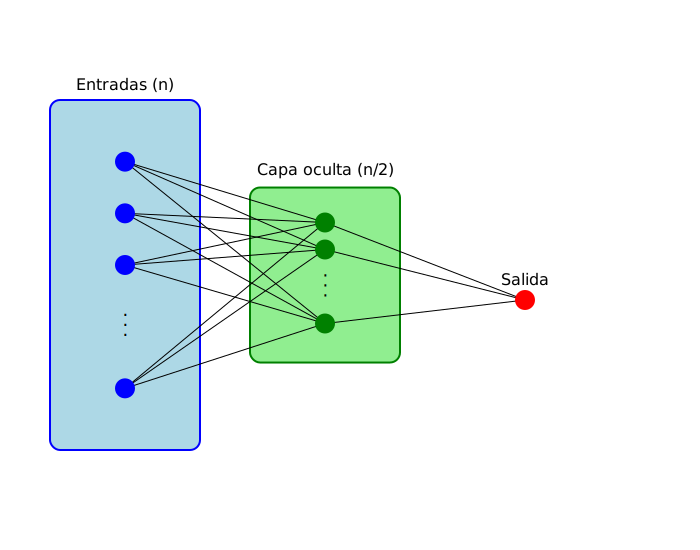
\includegraphics[width=\linewidth]{../Memoria/img/modelo/arquitecturas/arqnmediosBIN.pdf}
    \caption{MCB25.}
	    \end{minipage}
	    
	    \hspace{.5cm}
	        
	    \begin{minipage}{0.3\textwidth}
    			\centering
		    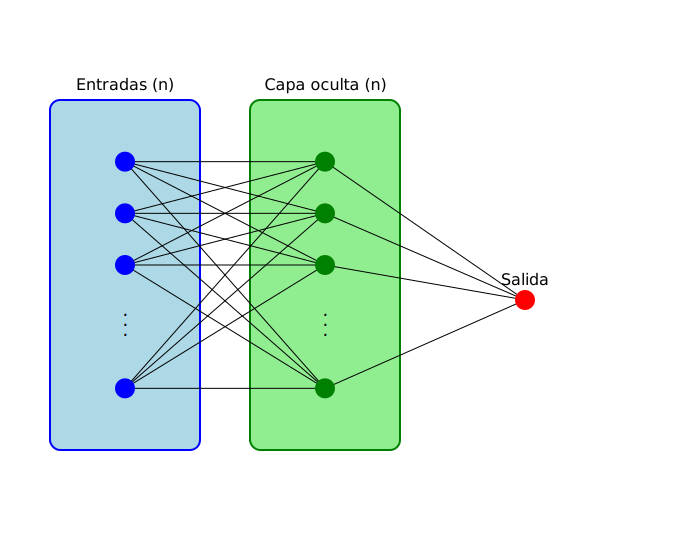
\includegraphics[width=\linewidth]{../Memoria/img/modelo/arquitecturas/arqnBIN.pdf}
		    \caption{MCB49.}
	    \end{minipage}	
	    \hspace{.5cm}
	        
	    \begin{minipage}{0.3\textwidth}
    			\centering
		    \includegraphics[width=\linewidth]{../Memoria/img/modelo/arquitecturas/arqnnBIN.pdf}
		    \caption{MCB98.}
	    \end{minipage}
	    }
	\end{figure}
	
\end{frame}


\begin{frame}{Arquitecturas desarrolladas para el MCM}
\begin{itemize}


	\item \textbf{MCM25}: Número de neuronas en la capa oculta igual a la mitad del número de atributos o entradas que recibe el modelo.
	\item \textbf{MCM49}: Número de neuronas en la capa oculta igual al mismo número de atributos o entradas que recibe el modelo.
	\item \textbf{MCM98}: Número de neuronas en la capa oculta igual al doble del número de atributos o entradas que recibe el modelo.
\end{itemize}
    	\begin{figure}[H]
	    \centering
	    \hbox{
	    \begin{minipage}{0.3\textwidth}
	    		\centering
		    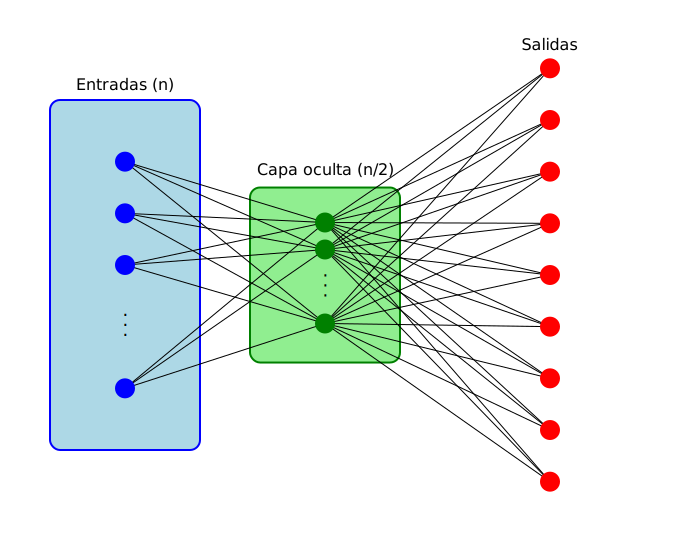
\includegraphics[width=\linewidth]{../Memoria/img/modelo/arquitecturas/arqnmediosMUL.pdf}
    \caption{MCM25.}
	    \end{minipage}
	    
	    \hspace{.5cm}
	        
	    \begin{minipage}{0.3\textwidth}
    			\centering
		    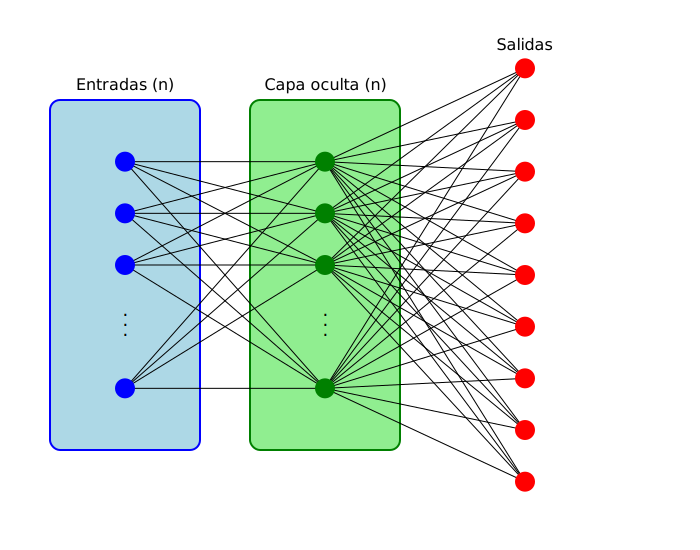
\includegraphics[width=\linewidth]{../Memoria/img/modelo/arquitecturas/arqnMUL.pdf}
		    \caption{MCM49.}
	    \end{minipage}	
	    \hspace{.5cm}
	        
	    \begin{minipage}{0.3\textwidth}
    			\centering
		    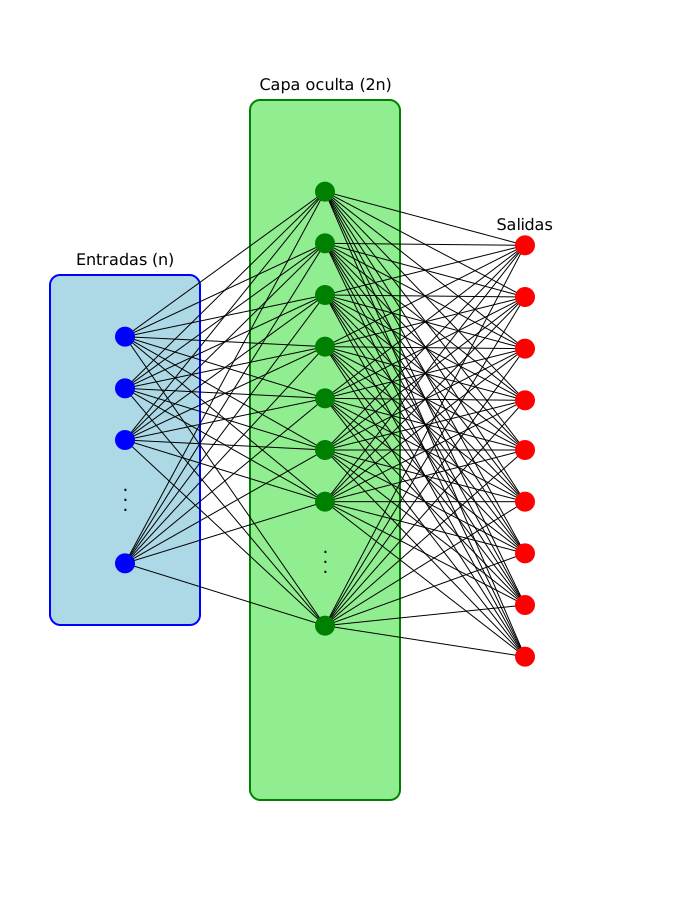
\includegraphics[width=\linewidth]{../Memoria/img/modelo/arquitecturas/arqnnMUL.pdf}
		    \caption{MCM98.}
	    \end{minipage}
	    }
	\end{figure}
	
\end{frame}


\subsection{Implementación de los modelos}
\begin{frame}{Validación cruzada}

	\begin{figure}
		\centering
	    \includegraphics[width=\linewidth]{./img/stratifiedkfolds.png}
    		\caption{Esquema de la validación cruzada (\textit{Stratificate k-fold} (5 \textit{folds}).}
	\end{figure}

\end{frame}

\begin{frame}{Implementación del MCB}
	\begin{itemize}
		\item \textbf{Función de pérdida}: \texttt{BCEWithLogistLoss}
		\item \textbf{Algoritmo de optimización}: \texttt{AdamW}
	\end{itemize}
	
%	\begin{figure}[H]
%	    \centering
%	    \includegraphics[width=0.6\textwidth]{../Memoria/img/modelo/codigo/modeloBIN.png}
%	    	\caption{Definición de la clase del modelo de clasificación binaria.}
%   		\label{fig:modBIN}
%	\end{figure}
	
	\begin{table}[H]
		\centering 
		\resizebox{0.6\textwidth}{!}{
		\begin{tabular}{|c|c|}
		\hline
		\textbf{Hiperparámetro} & \textbf{Posibles valores} \\ \hline
		\textit{Batch size} & [2000, 10000, 15000, 20000] \\ \hline
		\textit{Learning rate} & [$10^{-2}$, $10^{-3}$, $10^{-4}$] \\ \hline
		Épocas & [10, 20, 30] \\ \hline
		\end{tabular}
		}
		\caption{Valores de los hiperparámetros utilizados en los experimentos del modelo de clasificación binaria.}
		\label{tab:hiperBIN}
	\end{table}
\end{frame}

\begin{frame}{Implementación del MCM}
	\begin{itemize}
		\item \textbf{Función de pérdida}: \texttt{CrossEntropyLoss}
		\item \textbf{Algoritmo de optimización}: \texttt{AdamW}
	\end{itemize}
	
%	\begin{figure}[H]
%	    \centering
%	    \includegraphics[width=0.6\textwidth]{../Memoria/img/modelo/codigo/modeloMUL.png}
%	    	\caption{Definición de la clase del modelo de clasificación multiclase.}
%    		\label{fig:modBIN}
%	\end{figure}
	
	\begin{table}[H]
		\centering 
		\resizebox{0.6\textwidth}{!}{
		\begin{tabular}{|c|c|}
		\hline
		\textbf{Hiperparámetro} & \textbf{Posibles valores} \\ \hline
		\textit{Batch size} & [32, 64, 128, 256, 512] \\ \hline
		\textit{Learning rate} & [$10^{-2}$, $10^{-3}$, $10^{-4}$, $10^{-5}$] \\ \hline
		Épocas & [30, 50, 80, 100] \\ \hline
		\end{tabular}
		}
		\caption{Valores de los hiperparámetros utilizados en los experimentos del modelo de clasificación multiclase.}
		\label{tab:hiperBIN}
	\end{table}
\end{frame}



\subsection{Selección de las configuraciones de los modelos}

\begin{frame}{Selección de los mejores MCB}
Los mejores resultados del MCB los obtuvo la arquitectura con el doble de neuronas en su capa oculta que atributos de entrada tiene el modelo.
\begin{columns}[b]
\begin{column}{0.7\textwidth}
\begin{table}[H]
		\resizebox{1\textwidth}{!}{
\begin{tabular}{|>{\columncolor[HTML]{E0FFFF}}l|c|c|c|c|c|}
\hline
Posicion\_EXP & 1º-MCB98 & 2º-MCB98 & 3º-MCB98 & 4º-MCB98 & 5º-MCB98 \\
\hline
\cellcolor[HTML]{E0FFFF}batch\_size & \cellcolor[HTML]{66ffa8}20000 & \cellcolor[HTML]{66ffa8}10000 & \cellcolor[HTML]{66ffa8}15000 & \cellcolor[HTML]{66ffa8}15000 & \cellcolor[HTML]{66ffa8}10000 \\
\cellcolor[HTML]{E0FFFF}epochs & \cellcolor[HTML]{b1bafb}10 & \cellcolor[HTML]{b1bafb}30 & \cellcolor[HTML]{b1bafb}30 & \cellcolor[HTML]{b1bafb}10 & \cellcolor[HTML]{b1bafb}20 \\
\cellcolor[HTML]{E0FFFF}learning\_rate & \cellcolor[HTML]{f99595}$10^{-2}$ & \cellcolor[HTML]{f99595}$10^{-3}$ & \cellcolor[HTML]{f99595}$10^{-3}$ & \cellcolor[HTML]{f99595}$10^{-2}$ & \cellcolor[HTML]{f99595}$10^{-3}$ \\
\cellcolor[HTML]{E0FFFF}avg\_f1 & 0.998124 & 0.997941 & 0.997771 & 0.998015 & 0.997730 \\
\cellcolor[HTML]{E0FFFF}avg\_fn & 18.4 & 21.6 & 22 & 22.4 & 22.6 \\
\cellcolor[HTML]{E0FFFF}avg\_fp & 36.8 & 39 & 43.6 & 36 & 44.2 \\
\cellcolor[HTML]{E0FFFF}avg\_precision & 0.997501 & 0.997351 & 0.997039 & 0.997554 & 0.996999 \\
\cellcolor[HTML]{E0FFFF}avg\_recall & 0.998749 & 0.998531 & 0.998504 & 0.998477 & 0.998463 \\
\cellcolor[HTML]{E0FFFF}avg\_roc\_auc & 0.999781 & 0.999777 & 0.999776 & 0.999773 & 0.999777 \\
\cellcolor[HTML]{E0FFFF}avg\_tn & 344127.4 & 344125.2 & 344120.6 & 344128.2 & 344120 \\
\cellcolor[HTML]{E0FFFF}avg\_tp & 14686.2 & 14683 & 14682.6 & 14682.2 & 14682 \\
\hline
\end{tabular}
}
    \caption{Mejores cinco configuraciones para el MCB98.}
    \label{fig:BINhs98}
\end{table}
\end{column}

\begin{column}{0.3\textwidth}
\begin{figure}[H]
    \centering
    \includegraphics[width=1\textwidth]{../Memoria/img/modelo/matrices_confusion/MC_ENT_MCB98.png}
    \caption{Matriz de confusión 1º MCB98.}
    \label{fig:MC_ENT_MCB98}
\end{figure}

\end{column}
\end{columns}
\end{frame}


\begin{frame}{Mejores 5 configuraciones del MCB}
En este modelo no se observa que la arquitectura influya especialmente en los resultados obtenidos.
\begin{figure}[H]
    \centering
    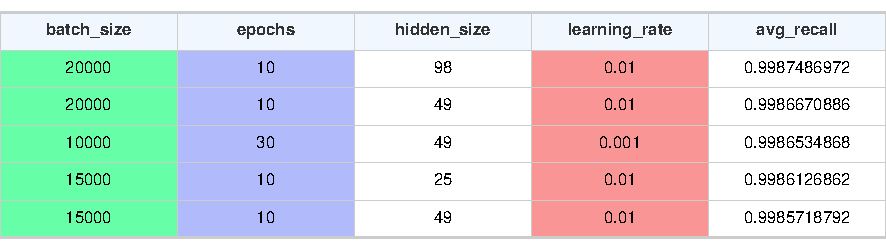
\includegraphics[width=0.85\textwidth]{../Memoria/img/modelo/resultados/BINtop5.pdf}
    \caption{Mejores cinco configuraciones de hiperparámetros del modelo de clasificación binaria.}
    \label{fig:BINtop5}
\end{figure}

\end{frame}




\begin{frame}{Selección de los mejores MCM}
Al igual que en el MCB, los mejores resultados del MCM se han obtenido en la arquitectura con el doble de neuronas en su capa oculta que atributos de entrada tiene el modelo.
\begin{columns}[b]
\begin{column}{0.6\textwidth}
\begin{table}[H]
		\resizebox{1\textwidth}{!}{
\begin{tabular}{|>{\columncolor[HTML]{E0FFFF}}l|c|c|c|c|c|}
\hline
Posicion\_EXP & 1º-MCM98 & 2º-MCM98 & 3º-MCM98 & 4º-MCM98 & 5º-MCM98 \\
\hline
\cellcolor[HTML]{E0FFFF}batch\_size & \cellcolor[HTML]{66ffa8}256 & \cellcolor[HTML]{66ffa8}256 & \cellcolor[HTML]{66ffa8}512 & \cellcolor[HTML]{66ffa8}64 & \cellcolor[HTML]{66ffa8}256 \\
\cellcolor[HTML]{E0FFFF}epochs & \cellcolor[HTML]{b1bafb}100 & \cellcolor[HTML]{b1bafb}80 & \cellcolor[HTML]{b1bafb}100 & \cellcolor[HTML]{b1bafb}80 & \cellcolor[HTML]{b1bafb}50 \\
\cellcolor[HTML]{E0FFFF}learning\_rate & \cellcolor[HTML]{f99595}$10^{-3}$ & \cellcolor[HTML]{f99595}$10^{-3}$ & \cellcolor[HTML]{f99595}$10^{-2}$ & \cellcolor[HTML]{f99595}$10^{-3}$ & \cellcolor[HTML]{f99595}$10^{-3}$ \\
\cellcolor[HTML]{E0FFFF}avg\_accuracy & 0.569414 & 0.556057 & 0.556915 & 0.556969 & 0.562083 \\
\cellcolor[HTML]{E0FFFF}avg\_f1\_macro & 0.413180 & 0.406773 & 0.388808 & 0.398720 & 0.397308 \\
\cellcolor[HTML]{E0FFFF}avg\_f1\_weighted & 0.583123 & 0.577553 & 0.574200 & 0.571020 & 0.569831 \\
\cellcolor[HTML]{E0FFFF}avg\_precision\_macro & 0.394898 & 0.385322 & 0.372836 & 0.377543 & 0.387029 \\
\cellcolor[HTML]{E0FFFF}avg\_precision\_weighted & 0.681971 & 0.675326 & 0.674534 & 0.669836 & 0.669688 \\
\cellcolor[HTML]{E0FFFF}avg\_recall\_macro & 0.577069 & 0.564962 & 0.573083 & 0.566046 & 0.550391 \\
\cellcolor[HTML]{E0FFFF}avg\_recall\_weighted & 0.569414 & 0.556057 & 0.556915 & 0.556969 & 0.562083 \\
\cellcolor[HTML]{E0FFFF}avg\_roc\_auc\_ovo & 0.813320 & 0.806782 & 0.809286 & 0.812789 & 0.800316 \\
\cellcolor[HTML]{E0FFFF}avg\_roc\_auc\_ovr & 0.788041 & 0.784984 & 0.781135 & 0.782758 & 0.777422 \\
\hline
\end{tabular}
}
    \caption{Mejores cinco configuraciones para el MCM98.}
    \label{fig:MULhs98}
\end{table}
\end{column}

\begin{column}{0.55\textwidth}
\begin{figure}[H]
    \centering
    \includegraphics[width=1\textwidth]{../Memoria/img/modelo/matrices_confusion/MC_ENT_MCM98.png}
    \caption{Matriz de confusión 1º MCM98.}
    \label{fig:MC_ENT_MCM98}
\end{figure}

\end{column}
\end{columns}
\end{frame}


\begin{frame}{Mejores 10 configuraciones del MCM}
En el caso del MCM, la arquitectura MCM98 ha obtenido en la fase de entrenamiento unos resultados muy superiores a las otras dos arquitecturas desarrolladas.
\begin{figure}[H]
    \centering
    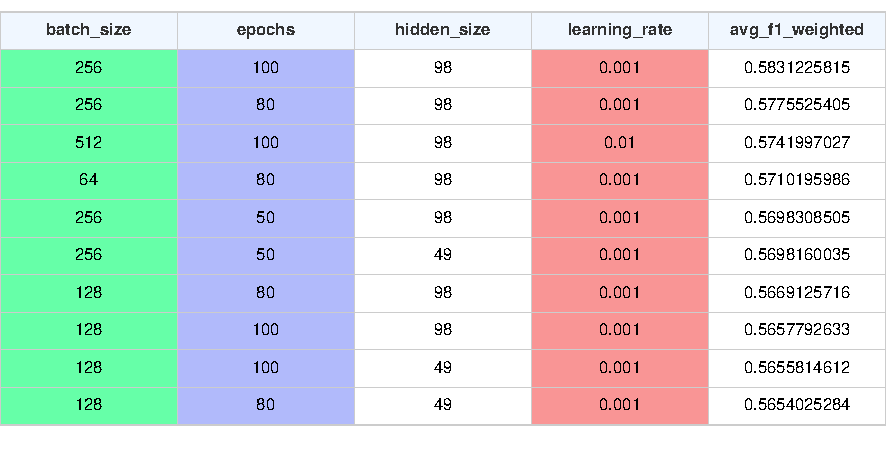
\includegraphics[width=1\textwidth]{../Memoria/img/modelo/resultados/MULtop10.pdf}
    \caption{Mejores diez configuraciones de hiperparámetros del modelo de clasificación multiclase.}
    \label{fig:BINtop5}
\end{figure}

\end{frame}






























\section{Evaluación}
Este capítulo se centra en la fase de evaluación de los modelos entrenados y correspondiente con la fase de evaluación de la metodología CRISP-DM. Se describe el conjunto de datos de prueba, el proceso de evaluación, la presentación de los resultados de las métricas y el análisis de las fortalezas y debilidades de los modelos.

\section{Conjunto de datos de prueba}
Para obtener el conjunto de datos para el entrenamiento de los modelos y el conjunto de datos de prueba, se ha de dividir el conjunto total de los datos, una vez que estos han sido preparados como siguiendo los pasos que se comentan en la Sección \ref{sec.prep-datos} \nameref{sec.prep-datos}. 


Al dividir el conjunto de datos, es crucial aplicar estratificación. Como se menciona en capítulos previos, esta técnica implica segmentar los datos de forma que se mantenga la misma distribución de clases en cada subconjunto. Esto resulta especialmente útil cuando las clases están desbalanceadas, ya que garantiza que todos los subconjuntos cuenten con una representación proporcional de cada clase, lo que mejora la precisión del modelo y minimiza los sesgos. Dado el desbalanceo observado en los datos de este trabajo, es esencial realizar una estratificación en cada división de los datos para evitar que algunas particiones contengan únicamente datos de una clase.


La división del conjunto de datos suele ser de en un 80\% para entrenamiento y un 20\% para evaluación, esta división se fundamenta en la necesidad de proporcionar suficiente cantidad de datos para que el modelo aprenda de manera efectiva, mientras se mantiene un conjunto de datos no utilizado en el entrenamiento para evaluar su rendimiento generalizando. La proporción del 80\% se considera adecuada para capturar patrones significativos en el entrenamiento sin comprometer la capacidad de evaluar el modelo en datos no vistos, lo que permite estimar su desempeño en situaciones realistas. Esta práctica también ayuda a evitar el sobreajuste, garantizando que los resultados del modelo no dependa en exclusiva de los datos utilizados en el entrenamiento \cite{bishop2006pattern}.

Para realizar la división, se utiliza la función \texttt{train\_test\_split} de la biblioteca \texttt{sklearn. model\_selection}. Esta función recibe el conjunto de los atributos y de las etiquetas de todo el \textit{dataset} utilizado, una vez que sus datos han sido preparados. Además, esta función recibe el porcentaje de los datos que se desea reservar para la evaluación o la fase de test, como se comenta en el párrafo anterior, en este trabajo el $0.2$ sobre 1 de los datos se destinan a evaluar los modelos entrenados. Finalmente, se especifica una semilla para que los datos se organicen de manera aleatoria y se especifica que se desea estratificar siguiendo el conjunto de las etiquetas.

Una vez divididos los datos, se normalizan los datos de evaluación, se convierten a tensores el conjunto de los atributos de pruebas y el conjunto de las etiquetas y se crea con estos tensores la instancia de la clase \texttt{DatasetTFG} que se utilizará para evaluar los modelos.

\section{Proceso de evaluación}
En el proceos de búsqueda de las configuraciones de hiperparámetros de los modelos con las que estos convergen mejor hacia una solución más generalizada, se ha utilizado la validación cruzada como se comenta en la Sección \ref{subsec:conjdatent}. La validación cruzada se utiliza para encontrar los mejores hiperparámetros de un modelo debido a su capacidad para proporcionar una evaluación más robusta y confiable del rendimiento del modelo. Este método divide el conjunto de datos en varios subconjuntos, realizando múltiples entrenamientos y evaluaciones, lo que permite reducir el riesgo de sobreajuste a un subconjunto específico. Además, la validación cruzada maximiza el uso de los datos disponibles, lo que resulta especialmente útil cuando los datos son limitados. 

Una vez que se han encontrado los hiperparámetros óptimos, se utiliza todo el conjunto de datos de entrenamiento, es decir, el 80\% del conjunto de datos para entrenar los modelos finales. Esto se debe a que, al haber ajustado previamente los hiperparámetros, se considera que los modelos se encuentran en sus configuraciones más eficientes, lo cual maximiza sus capacidades de generalización al aprender de la mayor cantidad de datos posible. De este modo, se obtienen unos modelos más robusto antes de realizar la evaluación final sobre un conjunto de prueba independiente que no ha sido utilizado en el proceso de entrenamiento \cite{hastie2009elements}.

El procesos de evaluación consiste en proporcionar a los modelos entrenados con las configuraciones comentadas en los párrafos anteriores, los datos de evaluación que no han visto durante la fase de entrenamiento. Durante este proceso se recogen los resultados que se obtienen en función de la matriz de confusión correspondiente a cada modelo para posteriormente obtener las métricas con las que comparar el desempeño de los modelos.

\section{Resultados de las métricas en el proceso de evaluación}
Para comparar los resultados obtenidos en la fase de evaluación de las cinco mejores configuraciones de hiperparámetros de cada arquitectura de cada modelo, se utilizan las mismas métricas comentadas en las Secciones \ref{sec.metricas-bin} \nameref{sec.metricas-bin} y \ref{sec:metricas-mul} \nameref{sec:metricas-mul} correspondientemente.

Con el objetivo de que la interpretación de los datos sea más sencilla, se ha añadido a las siguientes figuras una columna con la posición del \textit{ranking} que ocupó cada configuración en la fase anterior.


\subsection{Resultados del modelo de clasificación binaria}
La métrica utilizada para establecer el orden en los siguientes \textit{rankings} de configuraciones para los modelos de clasificación binaria es la misma empleada durante la fase previa de búsqueda de las mejores configuraciones de hiperparámetros: el \textit{Recall}.

\subsubsection{MCB25: Modelo de clasifcación binaria con un tamaño de capa oculta igual a la mitad del número de atributos de entrada que recibe el modelo}
En la Tabla \ref{fig:EVALMCB25}, se muestran los resultados obtenidos durante las evaluaciones de las cinco configuraciones de hiperparámetros con mejor desempeño durante la fase de búsqueda mencionados en la Figura \ref{fig:BINhs25}. Corresponden con las mejores configuraciones para la arquitectura del modelo de clasificación binaria que posee un tamaño de capa oculta de 25 neuronas.

\begin{table}[H]
\begin{tabular}{|>{\columncolor[HTML]{E0FFFF}}l|c|c|c|c|c|}
\hline
Posicion\_EXP & 3º-MCB25 & 2º-MCB25 & 1º-MCB25 & 5º-MCB25 & 4º-MCB25\\
\hline
\cellcolor[HTML]{E0FFFF}batch\_size & \cellcolor[HTML]{66ffa8}20000 & \cellcolor[HTML]{66ffa8}10000 & \cellcolor[HTML]{66ffa8}15000 & \cellcolor[HTML]{66ffa8}2000 & \cellcolor[HTML]{66ffa8}20000 \\
\cellcolor[HTML]{E0FFFF}learning\_rate & \cellcolor[HTML]{f99595}0.01 & \cellcolor[HTML]{f99595}0.001 & \cellcolor[HTML]{f99595}0.01 & \cellcolor[HTML]{f99595}0.001 & \cellcolor[HTML]{f99595}0.01 \\
\cellcolor[HTML]{E0FFFF}epochs & \cellcolor[HTML]{b1bafb}10 & \cellcolor[HTML]{b1bafb}30 & \cellcolor[HTML]{b1bafb}10 & \cellcolor[HTML]{b1bafb}10 & \cellcolor[HTML]{b1bafb}20 \\
\cellcolor[HTML]{E0FFFF}test\_recall & 0.998749 & 0.998640 & 0.998586 & 0.998422 & 0.998368 \\
\cellcolor[HTML]{E0FFFF}test\_accuracy & 0.999831 & 0.999813 & 0.999824 & 0.999826 & 0.999826 \\
\cellcolor[HTML]{E0FFFF}test\_f1 & 0.997934 & 0.997717 & 0.997853 & 0.997879 & 0.997879 \\
\cellcolor[HTML]{E0FFFF}test\_f2 & 0.998423 & 0.998271 & 0.998292 & 0.998205 & 0.998172 \\
\cellcolor[HTML]{E0FFFF}test\_precision & 0.997121 & 0.996796 & 0.997121 & 0.997337 & 0.997391 \\
\cellcolor[HTML]{E0FFFF}test\_roc\_auc & 0.999765 & 0.999772 & 0.999841 & 0.999818 & 0.999899 \\
\cellcolor[HTML]{E0FFFF}test\_specificity & 0.999877 & 0.999863 & 0.999877 & 0.999886 & 0.999888 \\
\hline
\end{tabular}
    \caption{Resultados de la evaluación del modelo de  clasificación binaria con \textit{n/2} neuronas en la capa oculta siendo \textit{n} el número de atributos de entrada.}
    \label{fig:EVALMCB25}
\end{table}


Los valores de la métrica \textit{Recall} obtenidos en las evaluaciones del modelo MCB25, son muy altos para todas las configuraciones y la diferencia entre sus valores es del orden de $1*10^{-4}$. Estas diferencias pueden deberse a circunstancias no controlables como el estado en el que se encontraba la máquina cuando se realizó la evaluación de los modelos o los pesos aleatorios iniciales que se eligieron en esa ejecución de los test.

La matriz de confusión de la mejor configuración de hiperparámetros obtenida en el 3º MCB25 durante su evaluación es la que se muestra en la Figura \ref{fig:MC_EVAL_MCB25}.

\begin{figure}[H]
    \centering
    \includegraphics[width=0.5\textwidth]{./img/evaluacion/matrices_confusion/MC_EVAL_MCB25.png}
    \caption{Matriz de confusión de la mejor configuración de hiperparámetros obtenida en el 3º MCB25 durante la fase de evaluación.}
    \label{fig:MC_EVAL_MCB25}
\end{figure}


\subsubsection{MCB49: Modelo de clasifcación binaria con un tamaño de capa oculta igual al número de atributos de entrada que recibe el modelo}
En la Tabla \ref{fig:EVALMCB49} se presentan los resultados obtenidos durante las evaluaciones de las cinco configuraciones de hiperparámetros con mejor desempeño, seleccionadas en la fase de búsqueda en la Figura \ref{fig:BINhs49} para la arquitectura del modelo de clasificación binaria que cuenta con una capa oculta de 49 neuronas.



\begin{table}[H]
\begin{tabular}{|>{\columncolor[HTML]{E0FFFF}}l|c|c|c|c|c|}
\hline
Posicion\_EXP & 2º-MCB49 & 1º-MCB49 & 5º-MCB49 & 3º-MCB49 & 4º-MCB49 \\
\hline
\cellcolor[HTML]{E0FFFF}batch\_size & \cellcolor[HTML]{66ffa8}10000 & \cellcolor[HTML]{66ffa8}20000 & \cellcolor[HTML]{66ffa8}2000 & \cellcolor[HTML]{66ffa8}15000 & \cellcolor[HTML]{66ffa8}2000 \\
\cellcolor[HTML]{E0FFFF}learning\_rate & \cellcolor[HTML]{f99595}0.001 & \cellcolor[HTML]{f99595}0.01 & \cellcolor[HTML]{f99595}0.0001 & \cellcolor[HTML]{f99595}0.01 & \cellcolor[HTML]{f99595}0.001 \\
\cellcolor[HTML]{E0FFFF}epochs & \cellcolor[HTML]{b1bafb}30 & \cellcolor[HTML]{b1bafb}10 & \cellcolor[HTML]{b1bafb}30 & \cellcolor[HTML]{b1bafb}10 & \cellcolor[HTML]{b1bafb}10 \\
\cellcolor[HTML]{E0FFFF}test\_recall & 0.998640 & 0.998640 & 0.998477 & 0.998477 & 0.998259 \\
\cellcolor[HTML]{E0FFFF}test\_accuracy & 0.999826 & 0.999835 & 0.999799 & 0.999835 & 0.999824 \\
\cellcolor[HTML]{E0FFFF}test\_f1 & 0.997880 & 0.997988 & 0.997554 & 0.997988 & 0.997852 \\
\cellcolor[HTML]{E0FFFF}test\_f2 & 0.998336 & 0.998379 & 0.998107 & 0.998281 & 0.998096 \\
\cellcolor[HTML]{E0FFFF}test\_precision & 0.997121 & 0.997338 & 0.996633 & 0.997500 & 0.997445 \\
\cellcolor[HTML]{E0FFFF}test\_roc\_auc & 0.999807 & 0.999843 & 0.999809 & 0.999898 & 0.999863 \\
\cellcolor[HTML]{E0FFFF}test\_specificity & 0.999877 & 0.999886 & 0.999856 & 0.999893 & 0.999891 \\
\hline
\end{tabular}
    \caption{Resultados de la evaluación del modelo de clasificación binaria con \textit{n} neuronas en la capa oculta siendo \textit{n} el número de atributos de entrada.}
    \label{fig:EVALMCB49}
\end{table}



Los valores de la métrica \textit{Recall} obtenidos durante las evaluaciones del modelo MCB49 son consistentemente altos para todas las configuraciones, y las diferencias entre ellos se encuentran en el orden de magnitud de $1*10^{-4}$. Estas variaciones podrían atribuirse a factores no controlables, como el estado del sistema al momento de la evaluación o la aleatoriedad en la inicialización de los pesos durante la ejecución de las pruebas.

La matriz de confusión correspondiente a la mejor configuración de hiperparámetros obtenida en el 2º MCB49 durante su evaluación se presenta en la Figura \ref{fig:MC_EVAL_MCB49}.

\begin{figure}[H]
    \centering
    \includegraphics[width=0.5\textwidth]{./img/evaluacion/matrices_confusion/MC_EVAL_MCB49.png}
    \caption{Matriz de confusión de la mejor configuración de hiperparámetros obtenida en el 2º MCB49 durante la fase de evaluación.}
    \label{fig:MC_EVAL_MCB49}
\end{figure}



\subsubsection{MCB98: Modelo de clasifcación binaria con un tamaño de capa oculta igual al doble del número de atributos de entrada que recibe el modelo}
La Tabla \ref{fig:EVALMCB98} muestra los resultados obtenidos en las evaluaciones correspondientes a las cinco configuraciones de hiperparámetros que presentaron el mejor desempeño durante la fase de búsqueda mostradas en al Figura \ref{fig:BINhs98}, aplicadas a la arquitectura del modelo de clasificación binaria con una capa oculta de 98 neuronas.
\begin{table}[H]
\begin{tabular}{|>{\columncolor[HTML]{E0FFFF}}l|c|c|c|c|c|}
\hline
Posicion\_EXP & 3º-MCB98 & 5º-MCB98 & 1º-MCB98 & 4º-MCB98 & 2º-MCB98 \\
\hline
\cellcolor[HTML]{E0FFFF}batch\_size & \cellcolor[HTML]{66ffa8}15000 & \cellcolor[HTML]{66ffa8}10000 & \cellcolor[HTML]{66ffa8}20000 & \cellcolor[HTML]{66ffa8}15000 & \cellcolor[HTML]{66ffa8}10000 \\
\cellcolor[HTML]{E0FFFF}learning\_rate & \cellcolor[HTML]{f99595}0.001 & \cellcolor[HTML]{f99595}0.001 & \cellcolor[HTML]{f99595}0.01 & \cellcolor[HTML]{f99595}0.01 & \cellcolor[HTML]{f99595}0.001 \\
\cellcolor[HTML]{E0FFFF}epochs & \cellcolor[HTML]{b1bafb}30 & \cellcolor[HTML]{b1bafb}20 & \cellcolor[HTML]{b1bafb}10 & \cellcolor[HTML]{b1bafb}10 & \cellcolor[HTML]{b1bafb}30 \\
\cellcolor[HTML]{E0FFFF}test\_recall & 0.998749 & 0.998749 & 0.998694 & 0.998477 & 0.998096 \\
\cellcolor[HTML]{E0FFFF}test\_accuracy & 0.999828 & 0.999822 & 0.999842 & 0.999833 & 0.999817 \\
\cellcolor[HTML]{E0FFFF}test\_f1 & 0.997907 & 0.997826 & 0.998070 & 0.997961 & 0.997770 \\
\cellcolor[HTML]{E0FFFF}test\_f2 & 0.998412 & 0.998379 & 0.998444 & 0.998270 & 0.997966 \\
\cellcolor[HTML]{E0FFFF}test\_precision & 0.997067 & 0.996905 & 0.997446 & 0.997446 & 0.997445 \\
\cellcolor[HTML]{E0FFFF}test\_roc\_auc & 0.999783 & 0.999770 & 0.999899 & 0.999899 & 0.999868 \\
\cellcolor[HTML]{E0FFFF}test\_specificity & 0.999874 & 0.999868 & 0.999891 & 0.999891 & 0.999891 \\
\hline
\end{tabular}
    \caption{Resultados de la evaluación del modelo de clasificación binaria con \textit{2n} neuronas en la capa oculta siendo \textit{n} el número de atributos de entrada.}
    \label{fig:EVALMCB98}
\end{table}

En las evaluaciones del modelo MCB98, los valores obtenidos para la métrica \textit{Recall} fueron elevados en todas las configuraciones, con diferencias del orden de $1*10^{-4}$. Estas pequeñas variaciones pueden explicarse por factores no controlables, como el estado del sistema en el momento de la evaluación o la inicialización aleatoria de los pesos durante la ejecución de las pruebas.


La matriz de confusión correspondiente a la mejor configuración de hiperparámetros obtenida en el 3º MCB98 durante su evaluación se presenta en la Figura \ref{fig:MC_EVAL_MCB98}.

\begin{figure}[H]
    \centering
    \includegraphics[width=0.5\textwidth]{./img/evaluacion/matrices_confusion/MC_EVAL_MCB98.png}
    \caption{Matriz de confusión de la mejor configuración de hiperparámetros obtenida en el 3º MCB98 durante la fase de evaluación.}
    \label{fig:MC_EVAL_MCB98}
\end{figure}




\subsection{Resultados del modelo de clasificación multiclase}
Para determinar el orden de los \textit{rankings} presentados a continuación, se emplea la misma métrica utilizada en la fase de búsqueda de configuraciones de hiperparámetros para los modelos de clasificación multiclase: el \textit{F1-weighted}.

\subsubsection{MCM25: Modelo de clasifcación multiclase con un tamaño de capa oculta igual a la mitad del número de atributos de entrada que recibe el modelo}

En la Tabla \ref{fig:EVALMCM25} se presentan los resultados obtenidos durante las evaluaciones de las cinco configuraciones de hiperparámetros con mejores métricas, identificadas durante la fase de búsqueda de hiperparámetros para la arquitectura del modelo de clasificación multiclase que cuenta con una capa oculta de 25 neuronas.

\begin{table}[H]
\begin{tabular}{|>{\columncolor[HTML]{E0FFFF}}l|c|c|c|c|c|}
\hline
Posicion\_EXP & 3º-MCM25 & 2º-MCM25 & 1º-MCM25 & 4º-MCM25 & 5º-MCM25 \\
\hline
\cellcolor[HTML]{E0FFFF}batch\_size & \cellcolor[HTML]{66ffa8}128 & \cellcolor[HTML]{66ffa8}512 & \cellcolor[HTML]{66ffa8}64 & \cellcolor[HTML]{66ffa8}256 & \cellcolor[HTML]{66ffa8}128 \\
\cellcolor[HTML]{E0FFFF}learning\_rate & \cellcolor[HTML]{f99595}0.001 & \cellcolor[HTML]{f99595}0.001 & \cellcolor[HTML]{f99595}0.001 & \cellcolor[HTML]{f99595}0.001 & \cellcolor[HTML]{f99595}0.001 \\
\cellcolor[HTML]{E0FFFF}epochs & \cellcolor[HTML]{b1bafb}80 & \cellcolor[HTML]{b1bafb}100 & \cellcolor[HTML]{b1bafb}100 & \cellcolor[HTML]{b1bafb}80 & \cellcolor[HTML]{b1bafb}50 \\
\cellcolor[HTML]{E0FFFF}test\_f1\_weighted & 0.538465 & 0.529706 & 0.491948 & 0.490342 & 0.435692 \\
\cellcolor[HTML]{E0FFFF}test\_accuracy & 0.519667 & 0.498341 & 0.463631 & 0.458354 & 0.406536 \\
\cellcolor[HTML]{E0FFFF}test\_f1\_macro & 0.371639 & 0.340072 & 0.339593 & 0.333974 & 0.305804 \\
\cellcolor[HTML]{E0FFFF}test\_precision\_macro & 0.415200 & 0.384902 & 0.376401 & 0.374790 & 0.354471 \\
\cellcolor[HTML]{E0FFFF}test\_precision\_weighted & 0.681380 & 0.670107 & 0.642648 & 0.646698 & 0.640704 \\
\cellcolor[HTML]{E0FFFF}test\_recall\_macro & 0.356826 & 0.325361 & 0.327492 & 0.320251 & 0.293147 \\
\cellcolor[HTML]{E0FFFF}test\_recall\_weighted & 0.568975 & 0.553186 & 0.550136 & 0.550342 & 0.534025 \\
\cellcolor[HTML]{E0FFFF}test\_roc\_auc\_ovo & 0.878231 & 0.871589 & 0.871532 & 0.877010 & 0.870398 \\
\cellcolor[HTML]{E0FFFF}test\_roc\_auc\_ovr & 0.875697 & 0.868443 & 0.870934 & 0.874640 & 0.867136 \\
\hline
\end{tabular}
    \caption{Resultados de la evaluación del modelo de clasificación multiclase con \textit{n/2} neuronas en la capa oculta siendo \textit{n} el número de atributos de entrada.}
    \label{fig:EVALMCM25}
\end{table}

La Tabla \ref{fig:EVALMCM25} anterior evidencia una diferencia en los valores de la métrica de comparación considerablemente mayor que la observada para las mismas configuraciones durante la fase de búsqueda de hiperparámetros. En los cinco mejores modelos representados en la figura, las diferencias en la métrica \textit{F1-weighted} durante la fase de búsqueda se encuentran en el orden de $1*10^{-2}$, mientras que en la fase de evaluación alcanzan un orden de $1*10^{-1}$, lo que indica una discrepancias con respecto a los resultados observados en la búsqueda de hiperparáemtros de la fase de modelado.

La matriz de confusión de la mejor configuración de hiperparámetros obtenida en el 3º MCM25 durante su evaluación, es la que se muestra en la Figura \ref{fig:MC_EVAL_MCM25}.

\begin{figure}[H]
    \centering
    \includegraphics[width=0.8\textwidth]{./img/evaluacion/matrices_confusion/MC_EVAL_MCM25.png}
    \caption{Matriz de confusión de la mejor configuración de hiperparámetros obtenida con en el 3º MCM25 durante la fase de evaluación.}
    \label{fig:MC_EVAL_MCM25}
\end{figure}

Dado que los datos empleados para entrenar el modelo de clasificación multiclase presentan un elevado desbalance entre clases, se recurre a la funcionalidad de normalización de matrices de confusión de \texttt{wandb} para generar una representación visual más informativa que la mostrada en la Figura \ref{fig:MC_EVAL_MCM25}. Esta técnica permite observar de forma más clara el comportamiento del modelo en cada clase, independientemente de su frecuencia en los datos, tal y como se puede apreciar en la Figura \ref{fig:MCNorm_EVAL_MCM25}. Al comparar ambas figuras, destaca la alto porcentaje de aciertos en la clase 0 y 8 en la Figura \ref{fig:MCNorm_EVAL_MCM25} y los resultados menos precisos para la clase 3.

La normalización en \texttt{wandb} convierte los conteos absolutos de la matriz de confusión en proporciones por clase real, lo que facilita la comparación del rendimiento del modelo entre clases desbalanceadas.

\begin{figure}[H]
    \centering
    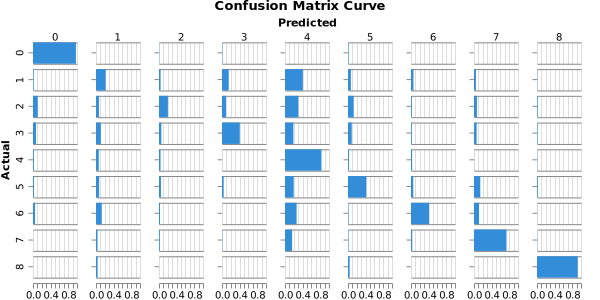
\includegraphics[width=0.95\textwidth]{./img/evaluacion/matrices_confusion/MCNorm_EVAL_MCM25.pdf}
    \caption{Matriz de confusión normalizada de la mejor configuración de hiperparámetros obtenida en el 3º MCM25 durante la fase de evaluación.}
    \label{fig:MCNorm_EVAL_MCM25}
\end{figure}



\subsubsection{MCB49: Modelo de clasifcación multiclase con un tamaño de capa oculta igual al número de atributos de entrada que recibe el modelo}
La Tabla \ref{fig:EVALMCM49} presenta los resultados de las evaluaciones realizadas sobre las cinco configuraciones de hiperparámetros con mejores métricas, seleccionadas durante la fase de búsqueda aplicada a la arquitectura del modelo de clasificación multiclase con una capa oculta compuesta por 49 neuronas.


\begin{table}[H]
\begin{tabular}{|>{\columncolor[HTML]{E0FFFF}}l|c|c|c|c|c|}
\hline
Posicion\_EXP & 5º-MCM49 & 4º-MCM49 & 3º-MCM49 & 2º-MCM49 & 1º-MCM49 \\
\hline
\cellcolor[HTML]{E0FFFF}batch\_size & \cellcolor[HTML]{66ffa8}256 & \cellcolor[HTML]{66ffa8}64 & \cellcolor[HTML]{66ffa8}128 & \cellcolor[HTML]{66ffa8}128 & \cellcolor[HTML]{66ffa8}256 \\
\cellcolor[HTML]{E0FFFF}learning\_rate & \cellcolor[HTML]{f99595}0.001 & \cellcolor[HTML]{f99595}0.001 & \cellcolor[HTML]{f99595}0.001 & \cellcolor[HTML]{f99595}0.001 & \cellcolor[HTML]{f99595}0.001 \\
\cellcolor[HTML]{E0FFFF}epochs & \cellcolor[HTML]{b1bafb}80 & \cellcolor[HTML]{b1bafb}50 & \cellcolor[HTML]{b1bafb}80 & \cellcolor[HTML]{b1bafb}100 & \cellcolor[HTML]{b1bafb}50 \\
\cellcolor[HTML]{E0FFFF}test\_f1\_weighted & 0.516647 & 0.501065 & 0.498233 & 0.467576 & 0.436878 \\
\cellcolor[HTML]{E0FFFF}test\_accuracy & 0.486589 & 0.461617 & 0.452423 & 0.429247 & 0.416081 \\
\cellcolor[HTML]{E0FFFF}test\_f1\_macro & 0.368803 & 0.325784 & 0.339188 & 0.316954 & 0.327882 \\
\cellcolor[HTML]{E0FFFF}test\_precision\_macro & 0.348930 & 0.326530 & 0.338391 & 0.327875 & 0.331214 \\
\cellcolor[HTML]{E0FFFF}test\_precision\_weighted & 0.657655 & 0.648645 & 0.671855 & 0.656385 & 0.651054 \\
\cellcolor[HTML]{E0FFFF}test\_recall\_macro & 0.560934 & 0.555375 & 0.572878 & 0.552602 & 0.534408 \\
\cellcolor[HTML]{E0FFFF}test\_recall\_weighted & 0.486589 & 0.461617 & 0.452423 & 0.429247 & 0.416081 \\
\cellcolor[HTML]{E0FFFF}test\_roc\_auc\_ovo & 0.883130 & 0.877907 & 0.887773 & 0.883284 & 0.875257 \\
\cellcolor[HTML]{E0FFFF}test\_roc\_auc\_ovr & 0.850867 & 0.848678 & 0.859088 & 0.847522 & 0.841436 \\
\hline
\end{tabular}
    \caption{Resultados de la evaluación del modelo de clasificación multiclase con \textit{n} neuronas en la capa oculta siendo \textit{n} el número de atributos de entrada.}
    \label{fig:EVALMCM49}
\end{table}

Al analizar los resultados obtenidos para esta arquitectura, destaca más allá del bajo rendimiento reflejado por la métrica \textit{F1-weighted}, el hecho de que el orden de las configuraciones se ha invertido respecto a lo observado en la fase de búsqueda. Las posibles causas de este comportamiento se detallan en la Sección \ref{sec:analEVAL}.

La matriz de confusión de la mejor configuración de hiperparámetros obtenida en el 5º MCM49 durante su evaluación, es la que se muestra en la Figura \ref{fig:MC_EVAL_MCM49}.

\begin{figure}[H]
    \centering
    \includegraphics[width=0.8\textwidth]{./img/evaluacion/matrices_confusion/MC_EVAL_MCM49.png}
    \caption{Matriz de confusión de la mejor configuración de hiperparámetros obtenida con en el 5º MCM49 durante la fase de evaluación.}
    \label{fig:MC_EVAL_MCM49}
\end{figure}

Dado el elevado desbalance entre clases en los datos utilizados para entrenar el modelo de clasificación multiclase, se emplea la funcionalidad de normalización de matrices de confusión de \texttt{wandb} para generar una representación visual más informativa que la presentada en la Figura \ref{fig:MC_EVAL_MCM49}. Esta técnica facilita la observación más clara del comportamiento del modelo en cada clase, independientemente de su frecuencia en los datos, como se puede observar en la Figura \ref{fig:MCNorm_EVAL_MCM49}. Comparando la Figura \ref{fig:MCNorm_EVAL_MCM25} con la figura de los datos normalizados del MCM49, se observa que como consecuencia del cambio de arquitectura, las prácticamente las predicciones para todas las clases han empeorado, a excepción de la clase 5 que ha obtenido mejores resultados que en el MCM25.

La normalización en \texttt{wandb} convierte los conteos absolutos de la matriz de confusión en proporciones por clase real, lo que facilita la comparación del rendimiento del modelo entre clases desbalanceadas.

\begin{figure}[H]
    \centering
    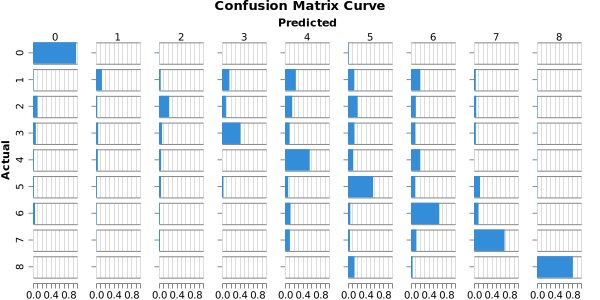
\includegraphics[width=0.95\textwidth]{./img/evaluacion/matrices_confusion/MCNorm_EVAL_MCM49.pdf}
    \caption{Matriz de confusión normalizada de la mejor configuración de hiperparámetros obtenida en el 5º MCM49 durante la fase de evaluación.}
    \label{fig:MCNorm_EVAL_MCM49}
\end{figure}




\subsubsection{MCB98: Modelo de clasifcación multiclase con un tamaño de capa oculta igual al doble del número de atributos de entrada que recibe el modelo}
En la Tabla \ref{fig:EVALMCM98} se ilustran los resultados obtenidos durante las evaluaciones correspondientes a las cinco configuraciones de hiperparámetros con mejores métricas, seleccionadas en la etapa de búsqueda de configuraciones para la arquitectura del modelo de clasificación multiclase con una capa oculta de 98 neuronas..

\begin{table}[H]
\begin{tabular}{|>{\columncolor[HTML]{E0FFFF}}l|c|c|c|c|c|}
\hline
Posicion\_EXP & 4º-MCM98 & 2º-MCM98 & 1º-MCM98 & 3º-MCM98 & 5º-MCM98 \\
\hline
\cellcolor[HTML]{E0FFFF}batch\_size & \cellcolor[HTML]{66ffa8}64 & \cellcolor[HTML]{66ffa8}256 & \cellcolor[HTML]{66ffa8}256 & \cellcolor[HTML]{66ffa8}512 & \cellcolor[HTML]{66ffa8}256 \\
\cellcolor[HTML]{E0FFFF}learning\_rate & \cellcolor[HTML]{f99595}0.001 & \cellcolor[HTML]{f99595}0.001 & \cellcolor[HTML]{f99595}0.001 & \cellcolor[HTML]{f99595}0.01 & \cellcolor[HTML]{f99595}0.001 \\
\cellcolor[HTML]{E0FFFF}epochs & \cellcolor[HTML]{b1bafb}80 & \cellcolor[HTML]{b1bafb}80 & \cellcolor[HTML]{b1bafb}100 & \cellcolor[HTML]{b1bafb}100 & \cellcolor[HTML]{b1bafb}50 \\
\cellcolor[HTML]{E0FFFF}test\_f1\_weighted & 0.568500 & 0.509088 & 0.506429 & 0.492392 & 0.465032 \\
\cellcolor[HTML]{E0FFFF}test\_accuracy & 0.545944 & 0.456177 & 0.447037 & 0.460094 & 0.424786 \\
\cellcolor[HTML]{E0FFFF}test\_f1\_macro & 0.375845 & 0.345703 & 0.339473 & 0.359955 & 0.315588 \\
\cellcolor[HTML]{E0FFFF}test\_precision\_macro & 0.365704 & 0.355874 & 0.368615 & 0.348133 & 0.324259 \\
\cellcolor[HTML]{E0FFFF}test\_precision\_weighted & 0.663088 & 0.690381 & 0.700087 & 0.646679 & 0.658504 \\
\cellcolor[HTML]{E0FFFF}test\_recall\_macro & 0.574354 & 0.583812 & 0.578126 & 0.573286 & 0.567694 \\
\cellcolor[HTML]{E0FFFF}test\_recall\_weighted & 0.545944 & 0.456177 & 0.447037 & 0.460094 & 0.424786 \\
\cellcolor[HTML]{E0FFFF}test\_roc\_auc\_ovo & 0.888441 & 0.890550 & 0.888079 & 0.879829 & 0.884775 \\
\cellcolor[HTML]{E0FFFF}test\_roc\_auc\_ovr & 0.865108 & 0.857470 & 0.859871 & 0.858953 & 0.847066 \\
\hline
\end{tabular}
    \caption{Resultados de la evaluación del modelo de clasificación multiclase con \textit{2n} neuronas en la capa oculta siendo \textit{n} el número de atributos de entrada.}
    \label{fig:EVALMCM98}
\end{table}

Los resultados obtenidos durante la fase de evaluación de esta arquitectura fueron significativamente inferiores a los alcanzados en la fase de búsqueda. Por ejemplo, en la quinta mejor configuración de hiperparámetros, la diferencia entre los resultados experimentales y los obtenidos en la evaluación es del orden de $1*10^{-1}$. Esta diferencia implica una reducción del 10\% en la precisión, o bien, un mayor número de errores en las clases con menor cantidad de muestras en comparación con la fase anterior.


La matriz de confusión de la mejor configuración de hiperparámetros obtenida en el 4º MCM98 durante su evaluación, es la que se muestra en la Figura \ref{fig:MC_EVAL_MCM98}.

\begin{figure}[H]
    \centering
    \includegraphics[width=0.8\textwidth]{./img/evaluacion/matrices_confusion/MC_EVAL_MCM98.png}
    \caption{Matriz de confusión de la mejor configuración de hiperparámetros obtenida en el 4º MCM98 durante la fase de evaluación.}
    \label{fig:MC_EVAL_MCM98}
\end{figure}

Debido al desbalanceo significativo entre las clases del conjunto de datos utilizados para entrenar el modelo de clasificación multiclase, se opta por utilizar la funcionalidad de normalización de matrices de confusión de \texttt{wandb}. Esta técnica permite generar una representación visual más clara que la mostrada en la Figura \ref{fig:MC_EVAL_MCM98}, facilitando así un análisis más preciso del comportamiento del modelo en cada clase, sin que este dependa de la frecuencia de las clases en los datos. Al comparar la Figura \ref{fig:MCNorm_EVAL_MCM98}, que corresponde con la versión normalizada del MCM98,  con las Figuras \ref{fig:MCNorm_EVAL_MCM49} y \ref{fig:MCNorm_EVAL_MCM25}, se percibe una mejora generalizada en la predicción de todas las clases. La única excepción es la clase 5, donde la arquitectura del MCM98 presenta peores resultados en comparación con el MCM25.

La normalización en \texttt{wandb} transforma los conteos absolutos de la matriz de confusión en proporciones por clase real, lo que simplifica la comparación del rendimiento del modelo, especialmente en situaciones con clases muy desbalanceadas.

\begin{figure}[H]
    \centering
    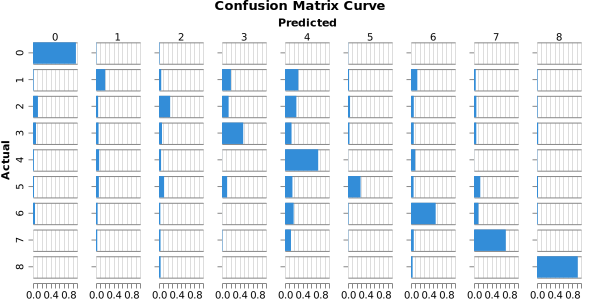
\includegraphics[width=0.95\textwidth]{./img/evaluacion/matrices_confusion/MCNorm_EVAL_MCM98.pdf}
    \caption{Matriz de confusión normalizada de la mejor configuración de hiperparámetros obtenida en el MCM98 durante la fase de evaluación.}
    \label{fig:MCNorm_EVAL_MCM98}
\end{figure}




\section{Análisis de los resultados obtenidos} \label{sec:analEVAL}
\subsection{Modelo de clasificación binaria}

Los resultados obtenidos durante la fase de búsqueda de las mejores configuraciones de hiperparámetros empleando validación cruzada \textit{k-fold} con estratificación muestran valores de \textit{Recall} consistentemente altos, todos por encima de $0{.}9985$, como se detalla en la Figura \ref{fig:BINtop5}. Este rendimiento indica una capacidad del modelo para identificar correctamente la clase mayoritaria de forma fiable y robusta en distintos subconjuntos de datos, lo cual respalda la estabilidad de las configuraciones seleccionadas durante esta fase de optimización \cite{bergstra2012random}.

Sin embargo, al aplicar estas mismas configuraciones en la fase de evaluación sobre un conjunto independiente (Figura \ref{fig:top5EVALMCB}), se observa una inversión parcial en el orden del rendimiento de las configuraciones. Algunas de las configuraciones con las mejores métricas en la búsqueda no mantienen su posición, mientras que otras ascienden en el \textit{ranking}. Este comportamiento puede atribuirse a pequeñas variaciones aleatorias en los datos o a la sensibilidad del modelo frente a distribuciones ligeramente diferentes, aun cuando estas diferencias se hayan mitigado mediante estratificación \cite{reimers2017optimal}.

A pesar de que las diferencias absolutas entre los valores de \textit{Recall} en ambas fases son reducidas (del orden de $1*10^{-4}$ a $1*10^{-3}$), su impacto puede ser relevante en tareas de clasificación binaria crítica, como la detección de conexiones maliciosas, donde incluso mínimas variaciones pueden traducirse en decisiones erróneas. El empeoramiento de algunas de las métricas puede deberse a factores como la inicialización aleatoria de pesos o el estado del sistema durante la inferencia, más que a un verdadero sobreajuste, dado que el proceso de validación cruzada ya controla adecuadamente este riesgo \cite{goodfellow2016deep}.

Asimismo, el análisis muestra que distintas combinaciones de \texttt{batch\_size}, \texttt{epochs}, \texttt{hidden \_size} y \texttt{learning\_rate} conducen a valores de \textit{Recall} muy próximos en evaluación. Esta convergencia en el rendimiento es coherente con estudios que sugieren que múltiples configuraciones en regiones planas del espacio de pérdida pueden llevar a modelos igualmente eficaces, especialmente en arquitecturas con un número de neuronal elevado como las utilizadas \cite{bouthillier2021sloppy}.

La observación de que varias configuraciones producen valores prácticamente idénticos de \textit{Recall} en la evaluación sugiere la presencia de una región de estabilidad en el espacio de soluciones. Sin embargo, el hecho de que estas configuraciones no coincidan con las mejor posicionadas en la búsqueda indica que, aunque la validación cruzada estratificada proporciona una estimación robusta, puede no capturar completamente la variabilidad inherente del conjunto de evaluación, especialmente si este presenta ligeras desviaciones de la distribución global \cite{recht2019imagenet}.

Los resultados reflejan un comportamiento coherente con lo esperado para modelos que han sido correctamente validados. Las diferencias encontradas entre fases no parecen ser estadísticamente significativas, pero sí lo suficientemente marcadas como para sugerir la conveniencia de utilizar estrategias complementarias de evaluación en futuros experimentos, como pruebas de sensibilidad o análisis de varianza.

\begin{figure}[H]
    \centering
    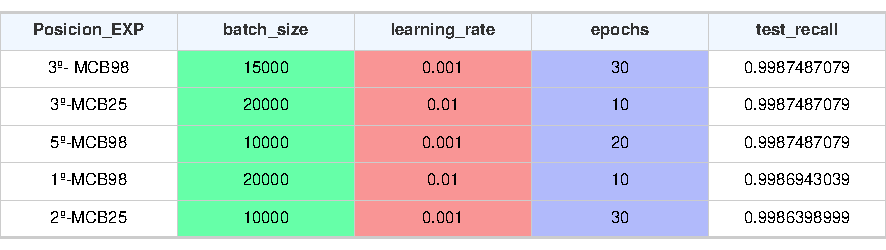
\includegraphics[width=0.9\textwidth]{./img/evaluacion/resultados/top5EVALMCB.pdf}
    \caption{Mejores cinco modelos en la fase de evaluación del modelo de clasificación binaria.}
    \label{fig:top5EVALMCB}
\end{figure}

\subsection{Modelo de clasificación multiclase}

Los resultados obtenidos durante la fase de búsqueda de hiperparámetros del modelo de clasificación multiclase (MCM), reflejados en la Figura \ref{fig:MULtop10}, indican valores moderados en las métricas utilizadas. En particular, el valor promedio de \textit{F1-weighted} se sitúa en torno a $0{.}57$, con ligeras variaciones entre las distintas configuraciones probadas. Este nivel de desempeño es coherente con la naturaleza desbalanceada del conjunto de datos, ya que el predominio de algunas clases afecta negativamente al promedio ponderado de precisión y \textit{Recall} \cite{he2009learning}.

Las métricas \textit{F1-macro} y \textit{Precision-macro} presentan valores sustancialmente más bajos que sus contrapartes ponderadas, lo que confirma que el modelo no logra un rendimiento equilibrado entre clases minoritarias y mayoritarias. Esta brecha sugiere que las clases menos representadas no son detectadas con suficiente eficacia, un fenómeno frecuente en escenarios de desbalance como el que se presenta en este trabajo, incluso al aplicar validación cruzada estratificada \cite{johnson2019survey}.

Al observar los resultados de la fase de evaluación (Figura \ref{fig:top5EVALMCM}), se constata que la métrica \textit{F1-weighted} no mejora significativamente respecto a la fase de búsqueda. De hecho, se observan valores incluso más bajos en algunas configuraciones, con un máximo de aproximadamente $0{.}568$ y un mínimo cercano a $0{.}509$. Este comportamiento sugiere que las configuraciones seleccionadas no generalizan adecuadamente al conjunto completo, a pesar de haber sido validadas mediante \textit{k-folds} \cite{reimers2017optimal}.

El análisis también muestra que el orden de las configuraciones en términos de rendimiento cambia entre ambas fases. Configuraciones que ocupaban posiciones intermedias o bajas durante la búsqueda escalan posiciones en la evaluación y viceversa. Esto podría estar relacionado con la distribución específica de las clases en el conjunto completo usado para la evaluación, el cual puede no coincidir exactamente con la distribución estratificada de los pliegues empleados durante la validación por circunstancias no controlables \cite{buda2018systematic}.

La pérdida de rendimiento observada puede explicarse también por el hecho de que, al entrenar con el conjunto completo en la evaluación, se pierde la ventaja del promedio sobre múltiples particiones que ofrece la validación cruzada. Esta situación puede inducir mayor varianza en los resultados y resaltar la sensibilidad del modelo a configuraciones particulares del entrenamiento \cite{dietterich1998approx}.

Por otra parte, el hecho de que el mejor resultado de \textit{F1-weighted} en evaluación ($0{.}568$) sea comparable al mejor valor obtenido en la búsqueda sugiere que el modelo alcanza un rendimiento máximo limitado por la naturaleza del problema. La estructura altamente desbalanceada del conjunto impone un techo al rendimiento global del modelo \cite{japkowicz2002class}.

A pesar de que el modelo 4º-MCM98 presenta una precisión global moderada (test\_accuracy $\approx$ 54.6 \%), sus valores de AUC, tanto en el enfoque \textit{One-vs-Rest} (0.8651) como en \textit{One-vs-One} (0.8884), indican una buena capacidad para distinguir entre las diferentes clases. Esto sugiere que el modelo, aunque no siempre acierta en la clase exacta, logra asignar puntuaciones de probabilidad adecuadas que reflejan correctamente la proximidad a la clase verdadera.


El modelo de clasificación multiclase presenta un rendimiento aceptable dadas las condiciones desbalanceadas del problema, pero revela claras limitaciones en la detección equilibrada de clases. Las discrepancias entre búsqueda y evaluación reflejan la dificultad del modelo para mantener un rendimiento robusto al exponerse a la totalidad del conjunto, y sugieren la necesidad de introducir nuevas estrategias no probadas en la Sección \ref{subsec:MCMdescart} \nameref{subsec:MCMdescart} orientadas al tratamiento explícito del desbalanceo de clases en futuras fases del desarrollo.

\begin{figure}[H]
    \centering
    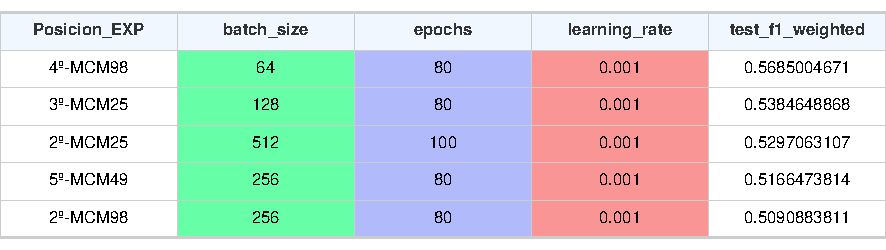
\includegraphics[width=0.9\textwidth]{./img/evaluacion/resultados/top5EVALMCM.pdf}
    \caption{Mejores cinco modelos en la fase de evaluación del modelo de clasificación multiclase.}
    \label{fig:top5EVALMCM}
\end{figure}

\section{Comparación de los resultados obtenidos con proyectos similares}

A continuación, se realiza una comparación entre los modelos propuestos en el presente trabajo y los desarrollados por \textit{Sarhan et al.}~\cite{sarhan2020netflow}, ambos aplicados a la detección de ataques en redes informáticas utilizando versiones del conjunto de datos \texttt{NF-UNSW-NB15-v3}.

\begin{itemize}
	\item Para el modelo de clasificación binaria, el respresentante de este trabajo será el que mejores resultados ha obtenido durante la fase de evaluación, el 3º-MCB98.
	\item Para el modelo de clasificación multiclase,el respresentante de este trabajo será el que mejores resultados ha obtenido durante la fase de evaluación, el 4º-MCM98. 
\end{itemize}


\subsection{Comparación de los modelos de clasificación binaria}

En la Tabla \ref{tab:compbin}, el modelo 3º-MCB98 evidencia una mejora sustancial en todas las métricas comparado con el modelo de \textit{Sarhan et al.}, destacando un aumento de $0.1479$ en el \textit{F1-Score} y más de cinco puntos porcentuales en el \textit{AUC}. Estas mejoras pueden atribuirse al uso de técnicas avanzadas de entrenamiento, ajuste de hiperparámetros y optimización de características.

\begin{table}[H]
\centering
\begin{tabular}{|l|c|c|c|c|c|c|}
\hline
\textbf{Modelo} & \textbf{\textit{Accuracy}} & \textbf{\textit{AUC}} & \textbf{\textit{F1-Score}} & \textbf{\textit{Recall}} & \textbf{\textit{Precision}} & \textbf{\textit{Specificity}} \\
\hline
\textit{Sarhan et al.} & 98.62\% & 0.9485 & 0.85 & -- & -- & -- \\
3º-MCB98 & 99.98\% & 0.9998 & 0.9979 & 0.9987 & 0.9971 & 0.9999 \\
\hline
\end{tabular}
\caption{Comparación de modelos de clasificación binaria.}
\label{tab:compbin}
\end{table}

\subsection{Comparación de los resultados por clase de los modelos de clasificación multiclase}

A pesar de que el modelo 4º-MCM98 no supera al de \textit{Sarhan et al.} en clases como \textit{Exploits} y \textit{Generic}, presenta un desempeño significativamente superior en \textit{Analysis} y \textit{Worms}. Estas diferencias que se pueden observar en la Tabla \ref{tab:compmulclass} pueden estar relacionadas con el preprocesamiento, la selección de características y la estrategia de balanceo utilizada mencionadas en el Capítulo \ref{cap.modelos}.

\begin{table}[H]
\centering
\begin{tabular}{|l|c|c|}
\hline
\textbf{Clase} & \textbf{\textit{F1-Score} (\textit{Sarhan et al.})} & \textbf{\textit{F1-Score} (4º-MCM98)} \\
\hline
Analysis (0) & 0.15 & 0.97 \\
Backdoor (1) & 0.17 & 0.20 \\
DoS (2) & 0.41 & 0.25 \\
Exploits (3) & 0.82 & 0.48 \\
Fuzzers (4) & 0.55 & 0.75 \\
Generic (5) & 0.66 & 0.28 \\
Reconnaissance (6) & 0.82 & 0.56 \\
Shellcode (7) & 0.75 & 0.72 \\
Worms (8) & 0.55 & 0.92 \\
\hline
\end{tabular}
\caption{Comparación de los valores obtenidos en \textit{F1-Score} por clase.}
\label{tab:compmulclass}
\end{table}


\subsection{Evaluación comparativa del rendimiento}
Tras observar las diferencias entre los valores de las métricas obtenidas en ambos proyectos, se puede asumir que:

\begin{itemize}
    \item El modelo 3º-MCB98 supera de forma consistente al modelo propuesto por \textit{Sarhan et al.} en todas las métricas evaluadas para la tarea de clasificación binaria.
  \item El modelo 4º-MCM98 destaca en clases con un menor número de muestras en el conjunto de datos utilizado para el entrenamiento como \textit{Analysis} y \textit{Worms}, mientras que el modelo de \textit{Sarhan et al.} muestra mayor estabilidad en clases con una mayor población de muestras. Esta diferencia puede deberse al uso de la función de pérdida ajustada utilizada en los modelos desarrollados en este proyecto, que penaliza con mayor severidad los errores en clases poco representadas, tal como se discute a lo largo del presente trabajo.
  
\end{itemize}


Los modelos desarrollados en este trabajo presentan mejoras notables en la clasificación binaria y un rendimiento competitivo en la clasificación multiclase. Aunque persisten desafíos en clases como \textit{Generic} y \textit{Exploits}, los resultados alcanzados en clases con relaciones de datos más complejas sugieren una mayor capacidad de generalización frente a los modelos publicados previamente.

\section{Despliegue}
Esta sección aborda la fase de despliegue de los modelos de clasificación binaria y multiclase desarrollados para la detección de conexiones malignas. La fase de despliegue en la metodología CRISP-DM implica la integración de los modelos entrenados en entornos operativos donde sus predicciones contribuyen a la toma de decisiones en tiempo real o en análisis periódicos, facilitando la detección automatizada y escalable de amenazas en redes como se comenta en capítulos anteriores \cite{wirth2000crisp}.

\section{Integración en entornos operativos}

Los modelos de clasificación binaria, orientados a distinguir conexiones malignas de benignas, y los modelos multiclase, diseñados para identificar diferentes categorías de conexiones malignas, deben ser implementados en plataformas que permitan la recepción continua de datos y procesamiento eficiente \cite{baylor2017tensorflow}. 

Para ello, es recomendable desplegarlos mediante APIs o microservicios, asegurando compatibilidad con sistemas de monitorización y respuesta automatizada. En el caso del modelo multiclase, la alta desproporción entre las clases y la naturaleza específica de los datos requieren especial atención en la validación en entorno real, dado que durante la fase de evaluación correspondiente con el capítulo \ref{cap.test} se utiliza el conjunto completo de datos y puede observarse degradación en desempeño frente a la fase de búsqueda \cite{gama2014survey}.

\section{Consideraciones técnicas}

El uso de validación cruzada estratificada durante la fase de búsqueda garantiza la estabilidad en la estimación de rendimiento, pero el despliegue debe contemplar la variabilidad inherente a datos nuevos y no vistos, especialmente en contextos dinámicos como la detección de conexiones malignas \cite{reimers2017optimal}. 

El ajuste adecuado de hiperparámetros, demostrado durante el capítulo \ref{cap.modelos}, debe ser preservado en producción, considerando limitaciones de hardware, latencia y volumen de datos. El control de versiones de los modelos es crucial para realizar actualizaciones y retrocesos en sus configuraciones de pesos, sin afectar a los resultados que devuelva el modelo \cite{peters2017machine}.

\subsection{Patrones arquitectónicos recomendados: Pipeline y Observador}

Para garantizar un despliegue robusto y adaptable de los modelos de clasificación en entornos operativos, lo recomendable es estructurar el sistema empleando patrones arquitectónicos que favorezcan la modularidad, la escalabilidad y la capacidad de respuesta ante eventos. Los patrones \textit{Pipeline} o Filtro Tuberia y Observador destacan como enfoques adecuados para satisfacer los requerimientos funcionales y no funcionales del sistema.

El patrón \textit{Pipeline} permite organizar el procesamiento de datos en una secuencia de etapas independientes, donde cada etapa representa una transformación o acción específica sobre el flujo de datos. Este enfoque favorece la separación de responsabilidades, facilita el mantenimiento, y permite escalar individualmente cada componente. Es particularmente útil para el procesamiento continuo de datos en tiempo real, como en entornos de detección de conexiones malignas \cite{neptune_ml_pipeline}.

Por otro lado, el patrón Observador resulta útil para implementar una arquitectura reactiva, en la cual distintos componentes del sistema (por ejemplo, sistemas de alerta, interfaces de usuario, módulos de registro) pueden suscribirse a los eventos generados por el modelo como la detección de una amenaza. Este patrón facilita una integración flexible entre los modelos de predicción y otros servicios que requieren actuar en función de los resultados generados, sin acoplamiento directo entre ellos \cite{gof_observer_pattern}.

La combinación de ambos patrones permite un diseño desacoplado, extensible y más mantenible, características fundamentales para sistemas de monitorización y respuesta en entornos dinámicos y críticos como la ciberseguridad.


\section{Monitorización y mantenimiento}
Una vez desplegados, los modelos requieren monitorización continua para detectar posibles cambios en la distribución de los datos o en el comportamiento de las conexiones, que puedan afectar el rendimiento del modelo (\textit{data drift} y \textit{concept drift}) \cite{gama2014survey}. En particular, para el modelo multiclase que ha sido entrenado con clases muy desbalanceadas, la monitorización de métricas como el \textit{F1-Weighted} es esencial para asegurar la calidad del diagnóstico en todas las categorías.

El mantenimiento de los modelos, incluye la recopilación de datos reales etiquetados, la reevaluación periódica del modelo y la posible reentrenamiento o ajuste de hiperparámetros para mantener la eficacia en la detección \cite{tsymbal2004problem}.

\section{Impacto y aplicación en el mundo real}

El despliegue efectivo de estos modelos contribuye a mejorar la seguridad en redes mediante la automatización de la detección de conexiones malignas, permitiendo respuestas rápidas y reducción de falsos positivos y negativos. La diferenciación entre múltiples tipos de conexiones malignas aporta un valor añadido para estrategias de mitigación específicas y optimización de recursos \cite{amershi2019software}.

La Figura \ref{fig:despliegue} muestra como podría implementarse de manera básica los modelos desarrollados en un entorno real de un sistema informático.

\begin{figure}[H]
    \centering
    \includegraphics[width=1\textwidth]{./img/despliegue/despliegue.pdf}
    \caption{Ejemplo de despliegue de los modelos en un sistema informático.}
    \label{fig:despliegue}
\end{figure}


\section{Conclusiones}
\begin{frame}{Conclusiones del proyecto}
	\begin{itemize}
		\item Se han desarrollado con éxito un modelo de clasificación binaria y un modelo de clasificación multiclase, capaces de detectar con gran precisión si una conexión a un sistema es benigna o maligna y de dar un clasificación previa del tipo de intrusión que se está produciendo.
		 \vspace{10mm}
		\item Tanto el MCB como el MCM son modelos basados en una red neuronal de tipo MLP (Perceptrón multicapa).
		 \vspace{10mm}
		\item Para el entrenamiento y la evaluación de los modelos se ha utilizado el \textit{dataset} \texttt{NF-UNSW-NB15-v3}, que está constituido por datos de origen semi-sintético.
	\end{itemize}
\end{frame}



\end{document}